\documentclass[conference]{IEEEtran}
\IEEEoverridecommandlockouts
% The preceding line is only needed to identify funding in the first footnote. If that is unneeded, please comment it out.
\usepackage[numbers]{natbib}
\usepackage{amsmath,amssymb,amsfonts}
\usepackage{algorithmic}
\usepackage{subcaption}
\usepackage{graphicx}
\usepackage{textcomp}
\usepackage{xcolor}
\def\BibTeX{{\rm B\kern-.05em{\sc i\kern-.025em b}\kern-.08em
    T\kern-.1667em\lower.7ex\hbox{E}\kern-.125emX}}
\begin{document}

\title{Availability Evaluation Models for Unmanned Aerial Vehicles (UAVs): One Analytical and One Numerical Method\\

\thanks{}
}

\author{\IEEEauthorblockN{1\textsuperscript{st} Luan Lins}
\IEEEauthorblockA{\textit{Centro de Informática} \\
\textit{Universidade Federal de Pernambuco}\\
Recife-PE, Brazil \\
lcsl2@cin.ufpe.br}
\and
\IEEEauthorblockN{2\textsuperscript{nd} Paulo Maciel}
\IEEEauthorblockA{\textit{Centro de Informática} \\
\textit{Universidade Federal de Pernambuco}\\
Recife-PE, Brazil \\
prrm@cin.ufpe.br}}

\maketitle

\begin{abstract}
%The reliability and availability evaluation of unmanned aerial vehicles (UAVs) is essential, especially when these are used to save lives. However, the infrastructure planning of the UAVs is not an easy task. Thus, the hierarchical modeling strategy may guide designers to evaluate and compare some results with already implemented proposals. This paper proposes a methodology and models to evaluate the availability of critical systems implemented in unmanned aerial vehicles. Two models are proposed: The first is an analytical model to evaluate availability metrics in the primary operating mode. The second model is a numerical method model with Petri nets to use redundancy mechanisms when improving the primary operational mode no longer has as much impact. The validation of the models takes place by comparing the results obtained with the real system using different scenarios. In this work, we present three case studies showing the use of the suggested technique to evaluate a UAV flight system, given the improvements and models used. The results show that it is possible to have an availability increase of 164.71\% in each technique and 193.82\% in mixed-use.

The reliability and availability evaluation of unmanned aerial vehicles (UAVs) is essential, especially when they are used to save lives. However, infrastructure planning of UAVs is not easy since they have small components and limited usable time. This paper proposes a methodology and models based on Stochastic Petri Nets and Markov chains to evaluate the availability of critical systems implemented in unmanned aerial vehicles. As these UAVs follow basic systems with one running drone and one spare drone, the hierarchical modeling strategy may guide designers in evaluating and comparing results with already implemented proposals. Furthermore, closed-form equations for steady-state availability are presented, allowing direct analytical solutions for large systems.

\medskip
Furthermore, the availability equations are symbolically differentiated, allowing parametric sensitivity analysis. The results of the sensitivity analysis enable system planning to improve steady-state availability. In this work, we present three case studies showing the use of the suggested technique to evaluate a UAV flight system, given the improvements and models used. The results show that it is possible to have an availability increase of 2.6x in each technique and almost 3x in mixed-use.
\end{abstract}

\begin{IEEEkeywords}
Modeling and Availability; Continuous Time Markov Chain; Stochastic Petri Net; Unmanned Aerial Vehicle (UAV);
\end{IEEEkeywords}

\section{Introduction}\label{sec:introduction}

The Internet of Things has been growing in recent years, increasing the number of connected devices around us. The global Internet of Things (IoT) market is estimated to grow from US \$800.00 billion by 2023 to US \$ 8,131.00 billion in 2030 at a compound annual growth rate (CAGR) of 20\% \citep{al2020internet}.

These devices constantly communicate and collect data that are analyzed and transformed into relevant information for decision-making that improves processes and people’s quality of life. These devices include smart home appliances, wearable devices, self-driving cars, industrial sensors and drones, also called unmanned aerial vehicles (UAVs), initially designed for combat. These very large UAVs have been equipped with bombs and guided by remote control over enemy lines.

Meanwhile, in recent years, unmanned aerial vehicles have become very popular because they can now move on their own, require less infrastructure and can be used in many fields. As a result, UAVs are being used for a variety of purposes beyond the military sector, such as surveillance\citep{basilico2015deploying}, smart agriculture \citep{lottes2017uav}, photogrammetry\citep{cesetti2011visual}, disaster management, public security\citep {maza2011experimental}, forest fire tracking \citep{pham2017distributed}, cloud monitoring \citep{renzaglia2016monitoring}, infrastructure supervision \citep{guerrero2013uav}, and power line inspection \citep{chang2017development}.

A percentage of UAVs also work with critical systems such as fire monitoring systems, air defense operations, and systems where continuous flights are required to maintain high monitoring availability, as they involve security, and failure could cause physical, personal, or financial damage. There is, therefore, a need for good planning of these systems to guarantee their efficiency.

%This article compares some availability criteria for critical systems implemented in unmanned aerial vehicles to support the planning and dimensioning of these systems. We propose an analytical model to evaluate availability metrics in the primary operating mode and a numerical method model with Petri nets to use redundancy mechanisms when improving the primary operating mode no longer has as much impact. We evaluated both scenarios based on sensitivity analysis to determine the best approach for the desired level of availability. 

Some works have studied the availability of UAV systems from the perspective of particular operational modes. \citet{Zaitseva2020, rusnak2019reliability} proposed a mathematical representation based on structure-function and reliability block diagrams (RBDs) of a fleet of UAVs and calculated their availability and reliability according to the failure time of the device and its control unit. \citet{Machida2021, Report} performed a trade-off analysis between availability, performance, and energy consumption in image processing using the fog (on a machine connected to an adjacent network) and edge (on the device) computing paradigms. Finally, \citet{Maccarthy2019} ] developed a stochastic analytical model for UAV system availability with cold-standby K-out-of-N redundancy. Although these works have addressed the availability of systems that use UAVs, most of them only address macro aspects using simple modeling approaches. We considered more detailed characteristics of the operation with UAVs, modeling the dependencies between the components and their background system. This work presents an availability model for system provisioning UAVs and a sensitivity assessment to identify components with the greatest negative influence on availability.

This article is structured as follows: Section \ref{sec:related_works} describes more recent work related to ours; Section \ref{sec:background} details the concepts of evaluation and performance, Markov chains, Petri nets, and sensitivity analysis used in this study; Section \ref{sec:methodology} describes the methodology used to carry out this study and the environment developed for the experiment. Analytical and numerical availability models are presented in detail in Section \ref{sec:model}. Section \ref{sec:case_studies} presents the case studies. Finally, in Section \ref{sec:conclusions}, conclusions are drawn from the article and some directions for future work are discussed.


\section{Related works}\label{sec:related_works}

Some authors have worked on unmanned aerial vehicles’ system availability in recent years. For example,  \citet{Petritoli2017, Petritoli2018} provides new ideas to increase the reliability of a UAV by optimizing maintenance activities. The reliability percentages assigned to each UAV system and subsystem are tracked to optimize time intervals and maintenance costs. However, redundancy mechanisms and availability models have yet to be proposed.

\citet{Zaitseva2020} and \citet{rusnak2019reliability} propose a mathematical representation of a fleet of UAVs based on the application of the structure-function of the system; this structure-function can be interpreted as a logical function. Although the system’s availability, reliability, and critical states are considered, this study deals with modeling a fleet of UAVs using reliability block diagrams as a basis. Therefore, it does not cover specific aspects of UAV operations, such as battery discharge, spare UAVs and batteries and changeover time between a failed UAV and a ready-to-operate UAV.

In \citet{Machida2021}, and \citet{Report} analyzed the trade-off between the availability, performance and power consumption of a drone image-processing system based on three different computing modes: single-drone computing mode, fog offloading and load balancing with another drone. The authors calculated the availability of the intelligent drone system based on a stochastic Petri net model. Although the authors use stochastic Petri nets to evaluate metrics such as availability and performance, in this study the authors only focus on computational processes and network link failures, where process failure can be caused by software defects or configuration error. Therefore, the authors do not consider the average time to failure and repair of the drone, the loading and unloading times, nor any general availability assessment model involving systems with redundancy mechanisms.

\citet{Maccarthy2019} developed an analytical stochastic model for system availability based on a Markov chain analysis for a K-out-of-N drone system. Among the model’s input parameters are the total number of drones, the number of drones in operation (drones in flight), the average repair time represented by the charging time, and the average failure time represented by the flight time reached by the drone. The author also performed a variability analysis of these parameters to find scenarios with greater system availability. However, the study did not separately model the drone and the power source or their redundancies, neither did their model include failure times and repairs to the rest of the system, such as the server, application, connection device or the drone itself, which could break down and be repaired in the middle of the operation.

As seen, most of the works presented to study the availability of UAV operational systems only address macro aspects of the availability of these systems, using simple modeling approaches. In our study, we considered more detailed aspects of the operation with UAVs, modeling the dependencies between the components and their background system. 

We propose two models, one with a Markov chain and the other with stochastic Petri nets, to represent a base operating system with UAVs characterized by 1 UAV in operation and another spare and 1 UAV in operation and N spares, illustrating a redundancy mechanism. Considering exponential times, we extracted the closed formula of the first model and performed a sensitivity analysis to find the system’s critical components, improve their times and evaluate them with these improvements separated into different case studies by models with and without redundancy mechanisms.



\section{Background}\label{sec:background}

\subsection{Reliability and Availability: An overview}
Dependability is a capacity in which a contracted system reliably produces a service. This idea emerged from the possibility of a breakdown of one or several system elements, preventing it from providing the service offered. Dependability is thus closely associated with reliability. The reliability of a system at a given moment is the probability of the system providing its service without failures up to $t$ time \citep{avizienis2004basic}. Hence, given the start value $0$ and the last value $t$ expressed by the wide interval, $[0,t)$, the reliability is the possibility of an element operating without failure in that period \citep{trivedi2008probability}. This equation (\ref{eq:01}) defines reliability.

\begin{align}\label{eq:01}
R = e^{\int_{0}^{t} \lambda(t')dt'},
\end{align}

Where $\lambda (t')$ is the immediate failure rate. If $\lambda (t') = t'\in (0,\infty)$, that is, constant, then the Time to Failure (TTF) is exponentially distributed with a failure rate equal to $\lambda$. Therefore,

\begin{align}
R(t) = e^{- \lambda t}.
\end{align}
 
Another significant dependability property is steady-state availability \citep{trivedi2008probability}.

We can use the Mean Time to Failure (MTTF) and the Mean Time To Repair (MTTR) to calculate the availability. Similarly, one can use the system Downtime and Uptime, as shown in Equations (3) and (4), respectively.

\begin{align}
A = \frac{E[Uptime]}{E[Uptime] + E[Downtime]}
\end{align}

\begin{align}
A = \frac{MTTF}{MTTF + MTTR}
\end{align}

The system's MTTF can be determined by the integral of reliability as a time function. In contrast, the MTTR of a system can be determined from MTTF's use to deliver the aspired availability. The availability is provided by (A), and unavailability is provided by $(UA= 1-A)$, as explained here.

\begin{align}
MTTF = \int_{0}^{t} R(t)dt.
\end{align}

When TTF is exponentially distributed with rate $\lambda$, then

\begin{align}
MTTF = \frac{1}{\lambda},
\end{align}

and,

\begin{align}
MTTF = MTTF \times (\frac{UA}{A}).
\end{align}

If TTF (Time to Failure) and TTR (Time to Repair) are exponentially distributed with $\lambda$ and $\mu$, respectively, then:

\begin{align}
A = \frac{\mu}{\mu + \lambda}.
\end{align}

\subsection{Markov Chain}

Markov models represent the interactions between various system components for descriptive and predictive purposes \citep{daniel2004performance}. The Markov process has been intensively adopted in performance and dependability modeling since around the 1950s \citep{maciel2012dependability}. Manufacturing, logistics, communication, and computer systems are some examples of fields that can rely on stochastic modeling as an interesting approach to address various problems \citep{maciel2021survey}.

A stochastic process is defined as a set of random variables $(\{ X_{i}(t):t \in T \})$ indexed through some parameter $(t)$. Each random variable $(X_i(t))$ is defined in a probability space. The parameter $t$ usually represents time, so $X_{i}(t)$ denotes the value assumed by the random variable at a time $t$. $T$  is called the parameter space and is a subset of $\mathbb{R}$ \citep{maciel2021survey}.

\subsection{Stochastic Petri Nets}

\begin{figure}[htbp]
\centerline{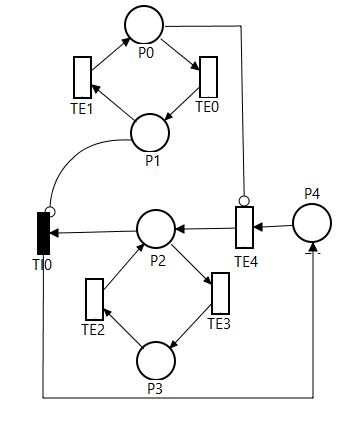
\includegraphics[scale=0.5]{img/cold-standby-example.png}}
\caption{Example of a cold standby model with Petri nets}
\label{fig:stochastic_petri_net_example}
\end{figure}

Petri nets (PN) denote a single large modeling mechanism that describes simultaneous, asynchronous, shared, parallel, deterministic, and stochastic processes \citep{german2000performance}. These nets determine a term procedure that provides a numerical and graphical description and have scientific tools that confirm the features and exactness of illustrated systems. An extension of PNs is denoted as Stochastic Petri Nets (SPNs) \citep{marsan1998modelling}. SPNs mate a stochastic stop with an individually clocked transition. Hence, stochastic Petri nets can be isomorphic in relation to continuous-time Markov chains (CTMC) and can give performance dimensions \citep{molloy1982integration}.

\subsection{Sensitivity analysis}

There are many methods for sensitivity analysis. Among them, we can stress \textit{Differential Sensitivity Analysis (PD)}, \textit{Sensitivity Measures One at a Time}, \textit{The Relative Deviation Method (RD)}, \textit{The Relative Deviation Rate (RDR)}, \textit{The partial rank correlation coefficient (PRCC)} and \textit{The Sensitivity Index (SI)} \citep{hamby1995comparison}. Our study will use the Sensitivity Index (SI), which uses the percentage difference technique for a simpler calculation.

The percentage difference technique for computing the sensitivity index $S_y(A)$ indicates the impact on a given availability caused by variations in an input parameter $y$. Equation 6 shows how the index of the sensitivity analysis is calculated for the y metric, where $max_y$ and $min_y$ represent the maximum and minimum output values, respectively, of the calculation, the parameter y varying up to  the maximum value $max_y$ \citep{clemente2022availability}.

\begin{align}\label{eq:sa}
S_y(A) = \frac{max_y - min_y}{max_y}.
\end{align}

During calculation of $S_y(A)$, the other parameters of the model need to be fixed. Thus, it is performed for all parameters to be calculated and to build the sensitivity analysis classification. This classification improves the predictability of increased availability.



\section{Proposed Methodology}\label{sec:methodology}

\begin{figure}[htbp]
\centerline{
\includegraphics[scale=0.9]{img/methodology.png}}
\caption{Methodology overview}
\label{fig:methodology}
\end{figure}

Figure \ref{fig:methodology} is a structure chart that summarizes our methodology. The rectangles represent each methodology step, and the arrows connecting the rectangles define the execution order.

In stages \textit{Studying the system} and \textit{Building metrics of interest}, we analyze the target system, seeking information from manufacturers and related work, and observing the system's operation to define metrics of interest. These steps supported the following steps:

In stage \textit{Building the models}, we build the models, and in stage \textit{Calculate the sensitivity rating and identify relevant components}, the sensitivity analysis is conducted \citep{maciel2017mercury, matos2020bottleneck, de2014redundant}. Then, in \textit{Results and suggestions}, we finally provide a rank that allows us to identify the components that need intervention. With this, we generate graphs simulating these improvements and redundancy mechanisms, varying the parameters used as input in the models and analyzing the impact on the metrics of interest. 

The models, assessments, and raw data can be seen and understood by designers, analysts, and administrators but hardly by senior management. Therefore, it is important to provide available graphical and textual interpretation to support the decision-making process\citep{melo2021distributed}. 


\section{Architecture and models}\label{sec:model}

This section will present the system's base architecture (its basic operational mode). Two models are conceived to represent the availability of the systems. A continuous-time Markov chain analytical model and the numerical method conceived through stochastic Petri nets.

\subsection{Proposed Architecture General System}

\begin{figure}[htbp]
\centerline{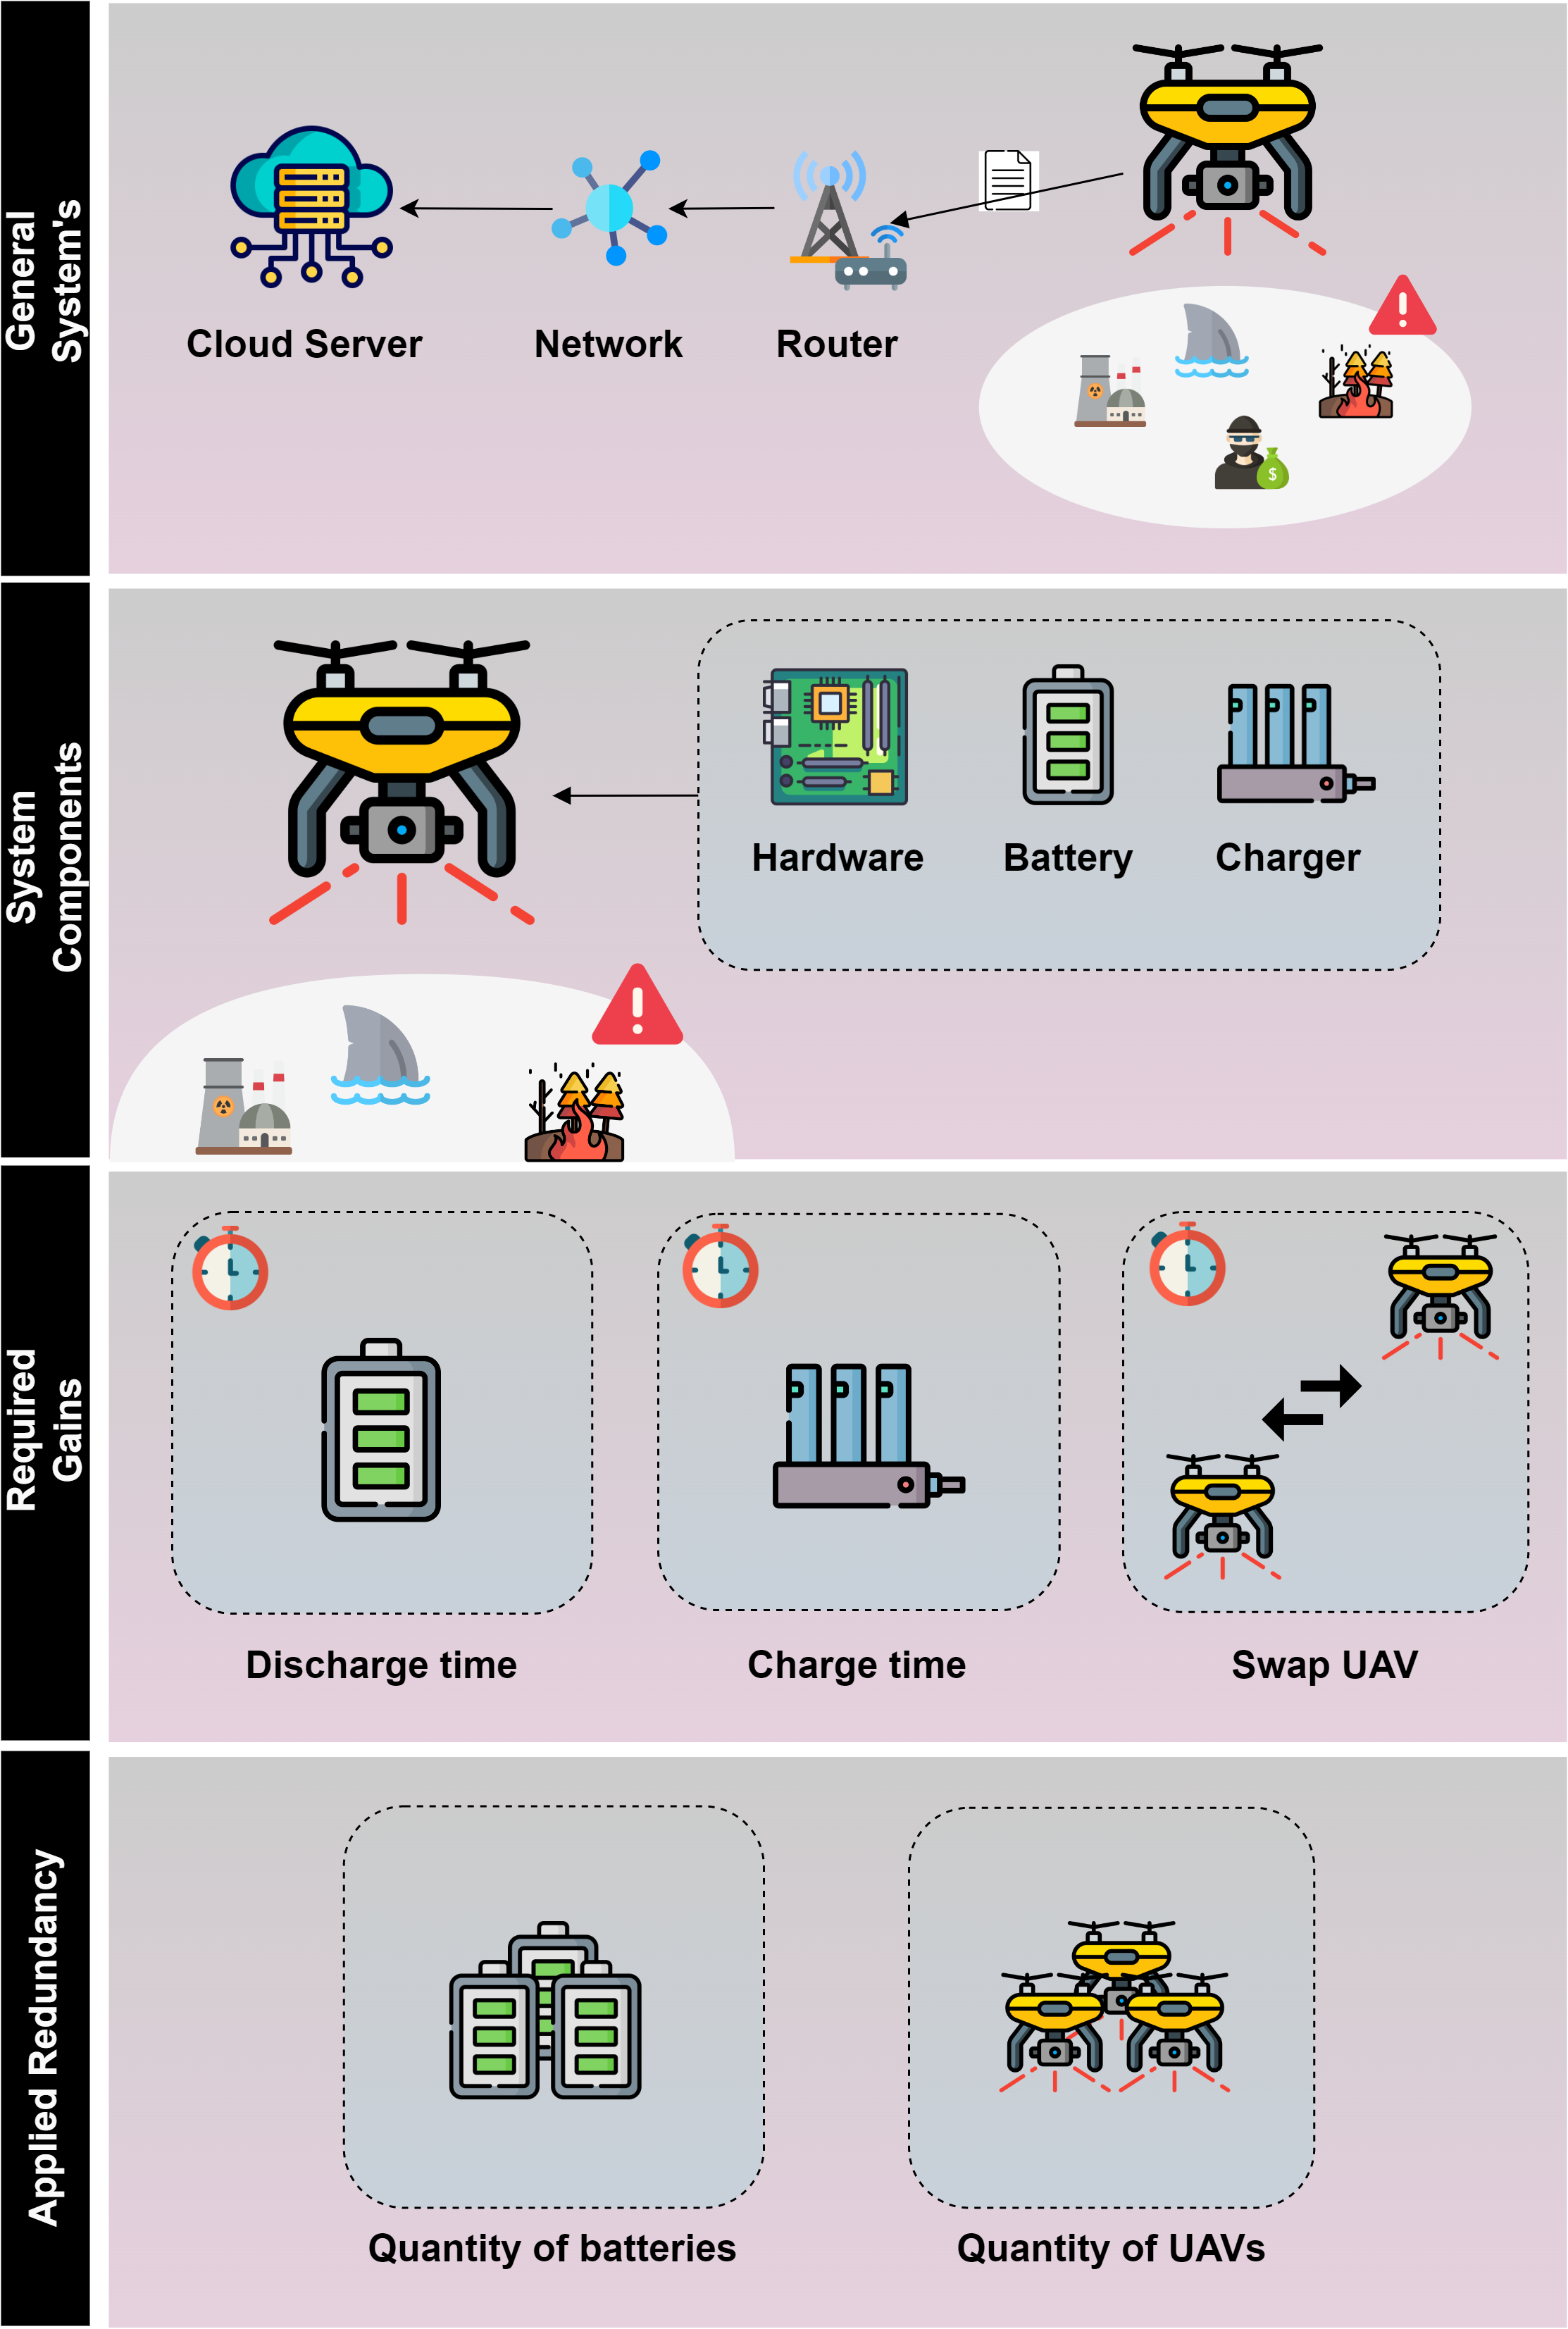
\includegraphics[scale=0.45]{img/operating_model.png}}
\caption{Overview of the Operating Mode}
\label{fig:operating_mode_overview}
\end{figure}

Figure \ref{fig:operating_mode_overview} presents an overview of the evaluated system and the studies employed, divided into \textit{General System}, \textit{System Components} of the UAV, \textit{Required Gains} and \textit{Redundancy Applied} to improve system availability.

In \textit{General System}, we have the system's basic functioning, a server for data processing; a UAV device for monitoring, and a router for the connection. The system is operational only if the server, router and UAV are working. For the UAV device, we assume that it is working if it is in flight.

\textit{System components}, shows the components of a UAV device that directly affect its availability, preventing increased flight times. The energy source (battery), charging system and UAV hardware are among them.

In \textit{Required Gains} and \textit{Applied Redundancy}, we have improvements in component times and UAV replacement (if considering redundancy methods) that can be applied to the base system to increase overall availability. It is important to note that the improvement in transition time is due to the development of an intelligent transition system that can trigger a reserve UAV before the active UAV returns to a landing base.

\subsection{CTMC baseline model}


\begin{figure}[htbp]
\centerline{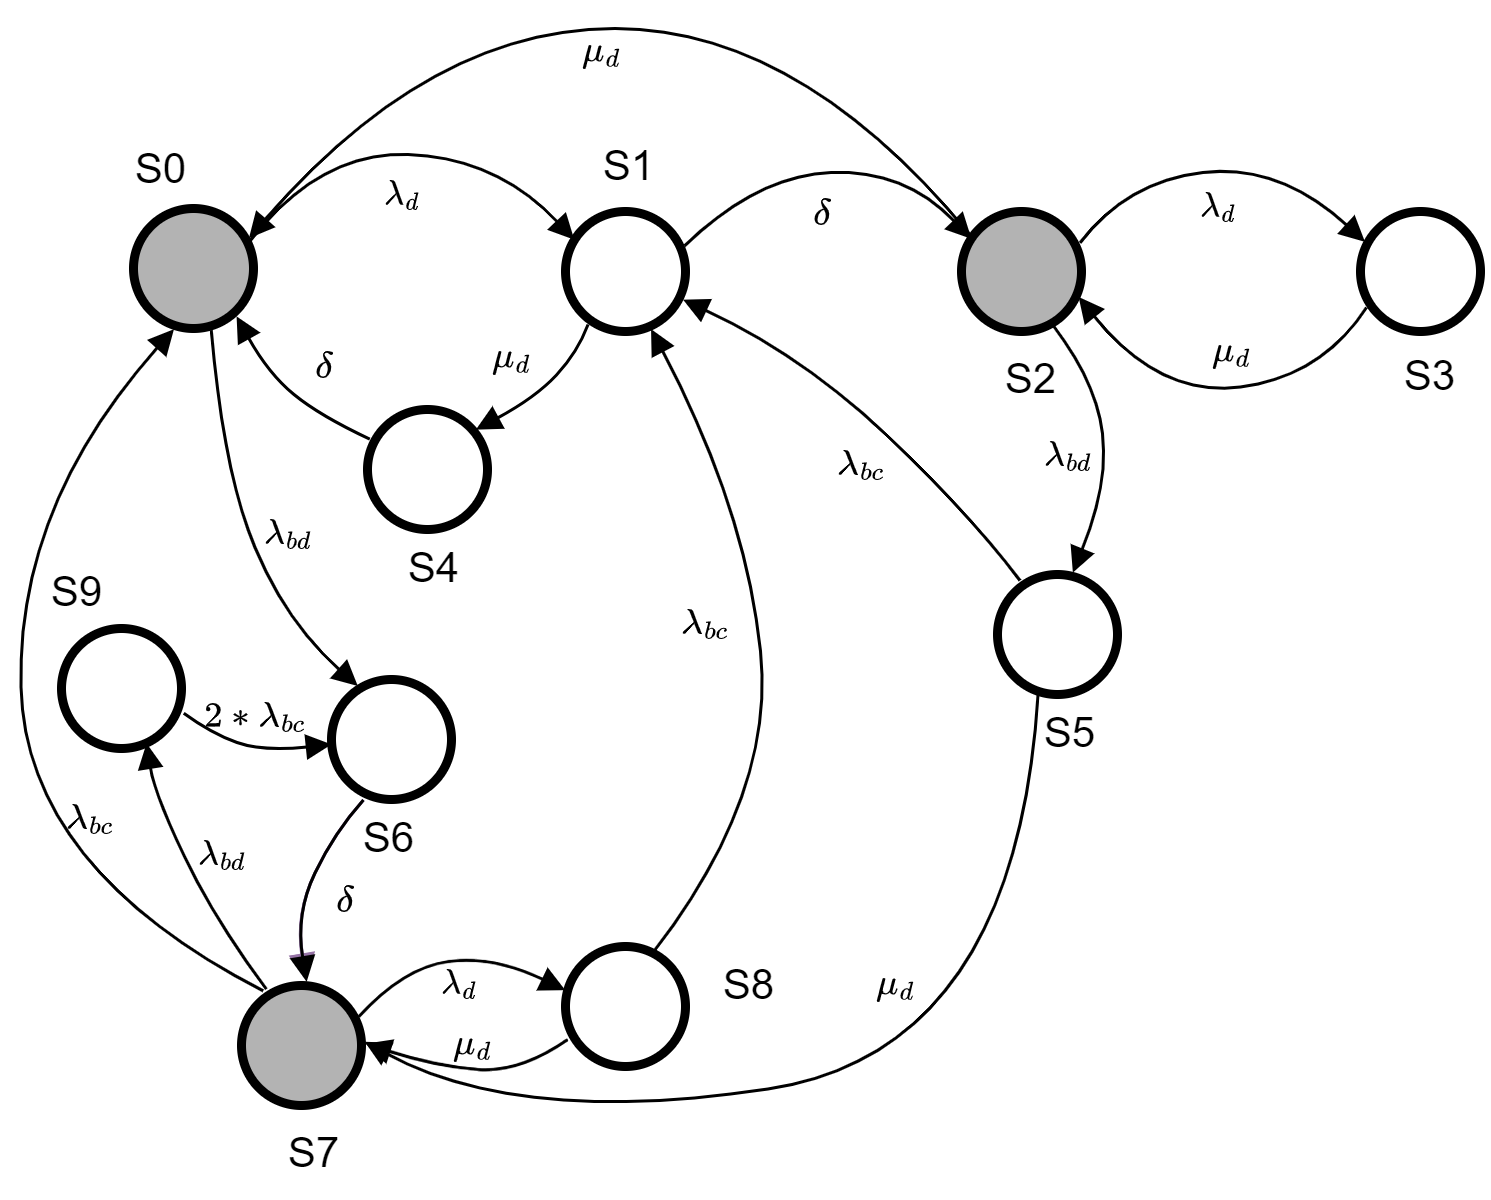
\includegraphics[scale=0.75]{img/CTMC_transparent.png}}
\caption{CTMC model of UAV flight system}
\label{fig:ctmc_model}
\end{figure}

\begin{table}[htbp]
\caption{Parameter Description for the CTMC model}
\begin{center}
\begin{tabular}{|c|c|}
\hline
\textbf{\textit{Parameter}}& \textbf{\textit{Description}} \\
\hline
  \(\lambda_{bd}\) & Battery discharge rate per hour \\
  \(\lambda_{bc}\)  & Battery charge rate per hour\\
 \(\mu_{d}\) & Drone repair rate per hour  \\
 \(\lambda_{d}\) & Drone failure rate per hour \\
 \(\delta\) & Drone swap rate per hour \\
\hline
\end{tabular}
\label{tab:ctmc_parameter_description}
\end{center}
\end{table}

Figure \ref{fig:ctmc_model} shows our continuous-time Markov chain model representing the flight system of the UAV device, consisting of a drone in operation (flying drone), a backup drone, and a backup power source. The model evaluates the availability of the flight system, having as input parameters the charging rate ($\lambda_{bc}$) and discharging rate($\lambda_{bd}$) of the drone battery per hour, as well as the rate of device hardware failure ($\mu_{d}$) and repair ($\lambda_{d}$) per hour. The exchange rate between the operating drone and a backup drone per hour is also considered in $\delta$; this exchange rate includes landing time, battery replacement, and takeoff for return (Table \ref{tab:ctmc_parameter_description}).

In the circle formula, we have the possible states being reached by the system; states illustrated in a dark color as the set of states $\{S0, S2, S7\}$ representing the operating system, that is, when at least one drone is flying over the area of interest or processing the information. Therefore, the other states represent the system offline, with some drones broken or unloaded and no drones or power sources to replace.

From this Markov chain model, we could extract the analytical model, which will serve as a basis for architects and designers in constructing a system with these characteristics. We are considering exponentially distributed times, which makes it possible to extract the closed formula illustrated by the equation \ref{eq:a_uav}.

\begin{align}\label{eq:a_uav}
A_{UAV} = \frac{\delta  \lambda_{bc} \mu_{d} (\alpha_{2} \delta \phi_{2} + \beta_{2} \mu_{d} \phi_{1})}{ \alpha_{2} \delta^{2} \theta_{2} + \lambda_{bc} \mu_{d} (\alpha_{3} \delta  \lambda_{bc} \lambda_{bd} \lambda_{d} + \theta_{1} \mu_{d})+ \beta_{2} \mu_{d}^{3} \phi_{3}}
\end{align}

Where: \\

\begin{minipage}{.8\textwidth}%  
\(\beta = \lambda_{bd} + \lambda_{d};\) \\
\(\beta_{2} = \lambda_{bd} + \mu_{d};\) \\
\(\beta_{3} = \lambda_{d} + \mu_{d};\) \\
\(\beta_{4} = \lambda_{bc} + \lambda_{bd};\) \\
\(\beta_{5} = \lambda_{bc} + \mu_{d};\) \\
\(\alpha_{1} = \beta + \lambda_{bc};\) \\
\(\alpha_{2} = \beta + \beta_{5};\) \\
\(\alpha_{3} = \beta_{3} + \beta_{4};\) \\
\(\alpha_{4} = \beta_{3}\lambda_{bc} + \lambda_{bd} \mu_{d};\) \\
\(\phi_{1} = \alpha_{1}\lambda_{bc} + \beta_{4} \mu_{d};\) \\
\(\phi_{2} = \beta_{3}\lambda_{bc} + \lambda_{bd} \mu_{d};\) \\
\(\phi_{3} = \beta \lambda_{bc}^{2} + \lambda_{bd} (\lambda_{bd} (\delta + \lambda_{bc}) + 2 \delta \lambda_{bc});\) \\
\(\phi_{4} = \beta_{3}^{2} + \beta_{3} (\lambda_{bc} + 3 \lambda_{bd}) + \lambda_{bd} (2 \lambda_{bc} + 3 \lambda_{bd});\) \\
\(\phi_{5} = \lambda_{d}^{2} + \lambda_{d} \mu_{d} + \mu_{d}^{2} ;\) \\
\(\theta_{1} = \alpha_{1} \beta  \beta_{2} \lambda_{bc} + 2 \beta  \beta_{2}  \delta \lambda_{bd}+ \delta  \lambda_{bc} \phi_{4};\) \\
\(\theta_{2} =  \alpha_{4} \lambda_{bd} \mu_{d} + \lambda_{bc}^{2} \phi_{5};\) \\
\end{minipage}%

We also include the formula for the availability of other components necessary for the functioning of a monitoring system like this, composed of a server and a connection device exemplified here as a router, its analytical formulas being shown in the equations \ref{eq:a_server} and \ref{eq:a_router}, respectively. However, we do not consider them in our sensitivity analyses and in assessing system availability. Components such as the server and the router have high availability compared to the UAV device, considered by us as the major bottleneck of the overall system and selected for availability improvement analysis.

\begin{align}\label{eq:a_server}
A_{Server} = \frac{\lambda_{hw}}{\lambda_{hw} + \mu_{hw}} \times \frac{\lambda_{os}}{\lambda_{os} + \mu_{os}} \times
\frac{\lambda_{hp}}{\lambda_{hp} + \mu_{hp}} 
\end{align}

\[\times(1- (\frac{\mu_{vm}}{\lambda_{vm} + \mu_{vm}})^{3})\]

\begin{align}\label{eq:a_router}
A_{R} = \frac{\lambda}{\lambda + \mu} 
\end{align}

The analytical model of server availability (Equation \ref{eq:a_server}) and router (Equation \ref{eq:a_router}) has in its structure the failure rate, represented by $\lambda$ and the repair rate $\mu $. However, the server availability model is composed of the product of the hardware availability models ($hw$), operating system ($os$), virtual machine management hypervisor ($hp$), and virtual machine model ($ vm$); components commonly used for processing a monitoring system.

\begin{align}\label{eq:a}
A = A_{Server} \times A_{R}  \times A_{UAV}
\end{align}

The system's general availability is given by Equation \ref{eq:a}, where we have the product of the server, router, and UAV flight system availability models.

\subsection{SPN redundancy model}

The UAV flight system availability analytical model (Equation \ref{eq:a_uav}) extracted from CTMC considers only the system in basic operating mode i.e. 1 in-flight UAV, 1 backup UAV, 1 backup battery. As already seen, we can use it to vary the failure and repair times of the UAV, battery, and recharging components to improve the availability metric. However, to include redundancy mechanisms in this model and have a system with a more advanced operating mode, we would have a model with a giant and unfeasible state space for calculating availability.

Given the problem of giant state space in Markov chains and analytical models extracted from it impossible for human calculation, we propose an approach with a numerical method model of stochastic Petri nets (SPN) that can be evaluated using computational tools such as Mercury \cite{maciel2017mercury}.

\begin{figure}[htbp]
\centerline{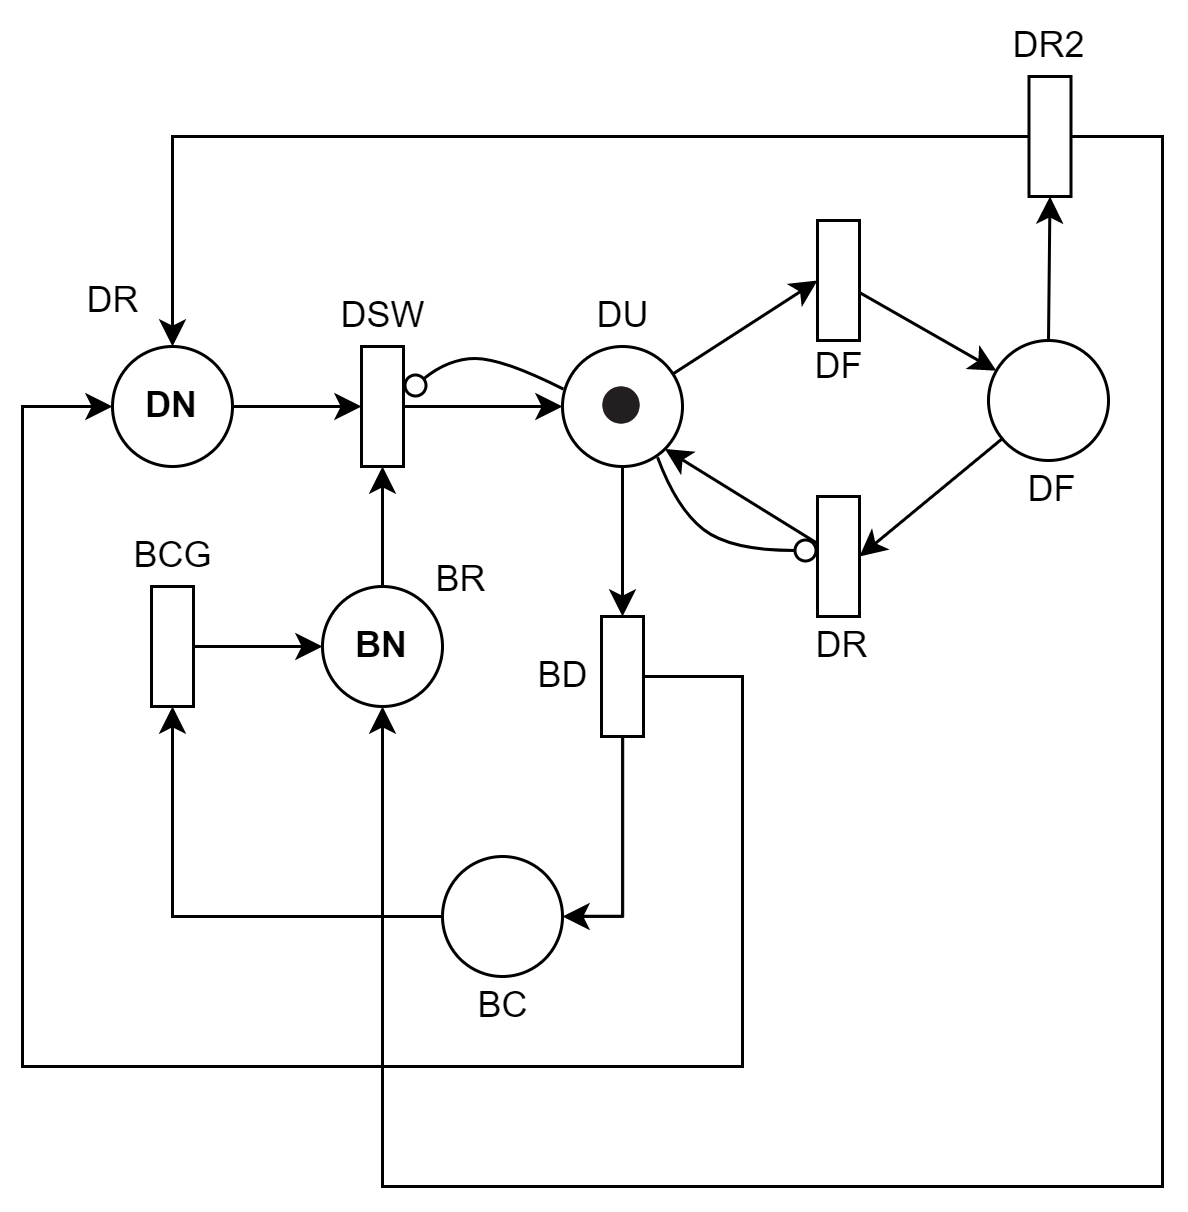
\includegraphics[scale=0.7]{img/SPN_transparent.png}}
\caption{SPN model of UAV flight system}
\label{fig:spn_model}
\end{figure}

\begin{table}[htbp]
\caption{Parameter Description for the SPN model}
\begin{center}
\begin{tabular}{|c|c|c|}
\hline
\textbf{\textit{Transition}} & \textbf{\textit{Parameter}}& \textbf{\textit{Description}} \\
\hline
 DF & MTTFD & Mean time to drone failure \\
 DR & MTTRD & Mean time to drone repair\\
 DR2 & MTTRD & With guard \textbf{$\#DU>0$} \\
 BD & MTTBD & Mean time to battery discharge \\ 
 BCG & MTTBC & Mean time to battery charge \\
 DSW & MTTSD & Mean time to swap drone \\
\hline
\end{tabular}
\label{tab:spn_parameter_description}
\end{center}
\end{table}

The SPN model represented by Figure \ref{fig:spn_model} was used to model the use of redundancy mechanisms in the system; its architecture is converted back to a CTMC state space but fully processed by the machine.

The place (circle) \textbf{DU} marks the system as working, while the place \textbf{DF} indicates a failed state. The other places: \textbf{DR}, \textbf{BR}, and \textbf{BC}, indicate the number of spare UAVs, spare batteries, and charging batteries, respectively.

Initially, 1 UAV is operational, with 1 backup UAV and one backup battery. The UAV has a mean time to failure (MTTF) and a mean time to repair (MTTR), as well as an average recharge, discharge, and swapping time. These times follow an exponential distribution, represented in the model by timed transitions (white rectangles) connected by arcs to the state places. All meantime parameters (MTTs) used as input to the model can be seen in Table \ref{tab:spn_parameter_description} per associated transition.

There are two types of arcs in the proposed model; the arc that ends with an arrow is the most common and indicates the activation of a transition if the requirements are met, and the movement of a token (the small black circle inside a place, which shows the number of features). In contrast, the arc that ends with a circle is called an inhibitor arc. An inhibitor arc indicates that a transition can only be activated if certain conditions are met. Timed transitions depend on the time to activate. The black rectangle is the transition called immediate transition, which can be activated if the required number of tokens is present in the connected location \citep{melo2021distributed}.



\section{Case studies}\label{sec:case_studies}
This section presents two case studies showing the use of each suggested technique to evaluate scenarios in an unmanned aerial vehicle (UAV) flight system. They are based on an analysis of availability and downtime measurements.

To start the evaluation with the models, we need to define the system parameter values in the basic operating mode (see section \ref{sec:model}). These values were collected from manufacturers' websites.

\textit{Case Study 1} 

Uses provided sensitivity analysis methodologies to identify parameters in drone flight system availability that require improvement.

\textit{Case Study 2} 

Assesses whether the sensitivity analysis performed in Case Study 1 significantly increases system availability and provides alternative redundancy mechanisms to achieve greater availability in the system's basic operating mode.

Finally, \textit{Case Study 3} uses the improvements of case study 1 in MTT parameters to apply redundancy mechanisms. The combination of the two methods used in Case Studies 1 and 2 can be considered when planning to evaluate a compromise between cost and availability. Designers and architects can choose to improve system components or increase their redundancy based on cost.

To guide ourselves on which rate or MTT of the system whose values could be varied first to obtain a better availability metric, we calculate a sensitivity ranking through the percentage differentiation technique defined by Equation \ref{eq:sa}, where the order of the parameter of the component reflects the significance of its impact on system availability (TABLE \ref{tab:sa_rank}).

\begin{table}[htbp]
\caption{Sensitivity ranking obtained}
\begin{center}
\begin{tabular}{|c|c|c|}
\hline
\textbf{\textit{Parameter}}& \textbf{\textit{Ranking}} & \textbf{\textit{Sensitivity index}} \\
\hline
\(\lambda_{bd}\) & \(1^{st}\) & -3.720460029055 \\
\(\lambda_{bc}\) & \(2^{nd}\) & 3.3226751100809997 \\
 \(\mu_{d}\) & \(3^{rd}\) & -1.064622392094 \\
\(\lambda_{d}\) & \(4^{th}\) & 0.9995887722079999 \\
\(\delta\) & \(5^{th}\) & 0.462793032533 \\
\hline
\end{tabular}
\label{tab:sa_rank}
\end{center}
\end{table}

In the sensitivity analysis performed, we have the battery discharge rate per hour as the parameter that most impacts the availability of the system according to the sensitivity index in column 3 of the table, followed by the charging rate per hour, repair rate, failure rate, and UAV exchange rate.

\subsection{Case Study 1}\label{sec:case_studies_sub01}

\begin{figure}[htbp]
\centerline{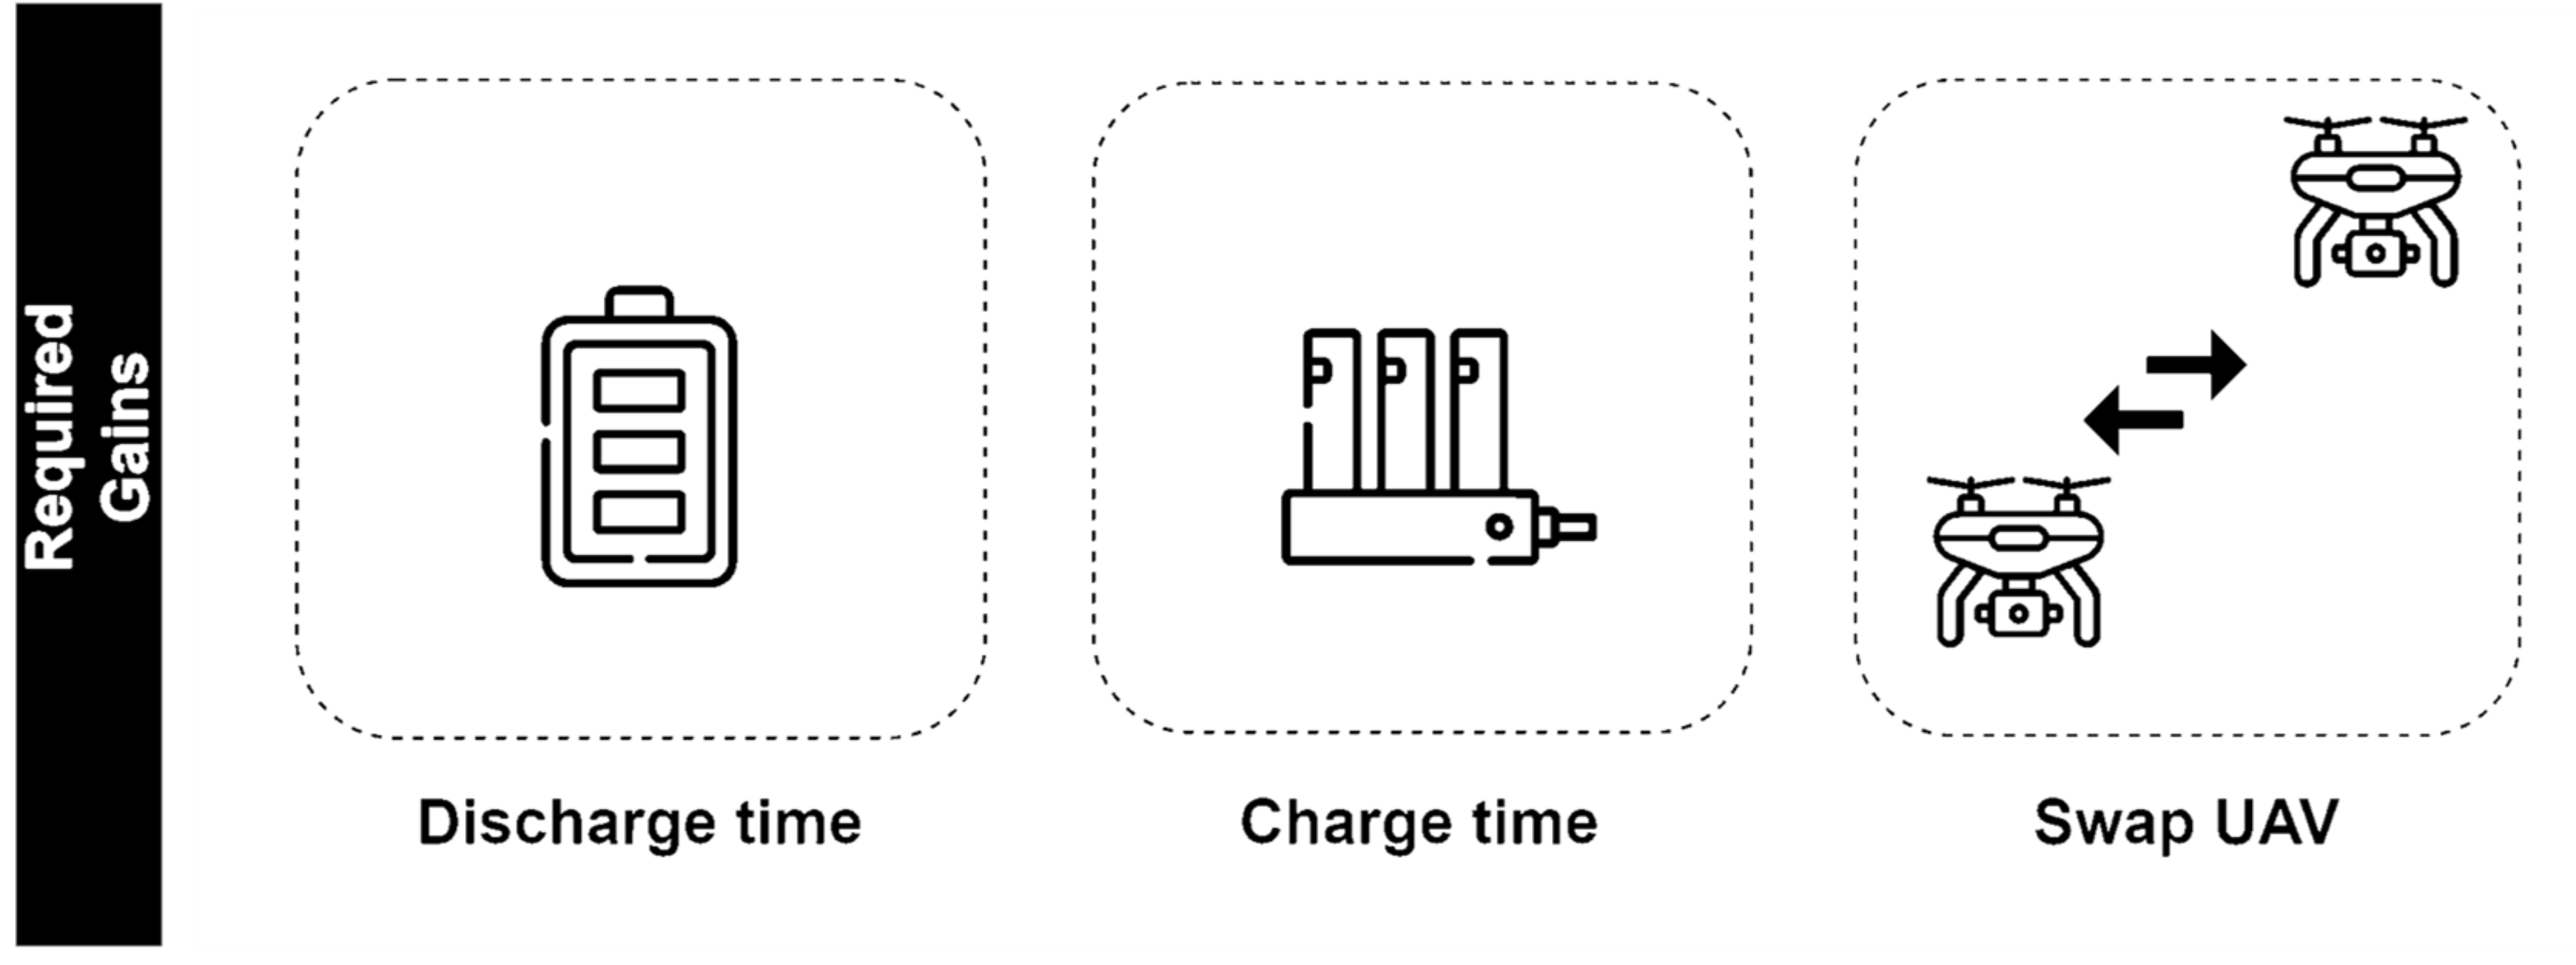
\includegraphics[scale=0.2]{img/operating_model_study_01.png}}
\caption{Required Gains}
\label{fig:case_study_01}
\end{figure}

In this case study, we use the analytical model and the CTMC flight system availability of UAV devices to increase availability by improving the input parameters. System baseline parameter values are shown in table \ref{tab:ctmc_parameter_values}, and variation graphs are in Figure \ref{fig:ctmc_sa}.



\begin{table}[htbp]
\caption{Parameter values for the CTMC model}
\begin{center}
\begin{tabular}{|c|c|}
\hline
\textbf{\textit{Parameter}} & \textbf{\textit{Value (rate)}} \\
\hline
  $\lambda_{bd}$  & 2 \\
  $\lambda_{bc}$   & 0.5 \\
  $\mu_{d}$   & 0.5  \\
  $\lambda_{d}$ & 0.0002 \\
  $\delta$  & 6 \\
\hline
\end{tabular}
\label{tab:ctmc_parameter_values}
\end{center}
\end{table}



Parameter values are given in rate format (amount per hour) for input to Markov chain and analytical models (section \ref{sec:background}). Where, $\lambda_{bd}$ is 2 (two) discharges per hour, $\lambda_{bc}$ is 0.5 (half) charge per hour, $\mu_{d}$ 0.5 (half) repair per hour, $\lambda_{d}$ is 0.0002 failures per hour, and $\delta$ is 6 UAV changes per hour.

Initially, we started our analysis by varying the value of $\lambda_{bd}$ (battery discharge rate), set this at an improved value, and varied the next one, the $\lambda_{bc}$ (charging rate). Finally, we varied the swap parameter ($\delta$) with $\lambda_{bd}$ and $\lambda_{bc}$ set to improved values. The UAV repair fee ($\mu_{d}$) and failure fee ($\lambda_{d}$) values were not changed since their baseline values had little impact on overall availability.

\begin{figure}[htbp]
     \centering
     \begin{subfigure}[b]{0.45\textwidth}
         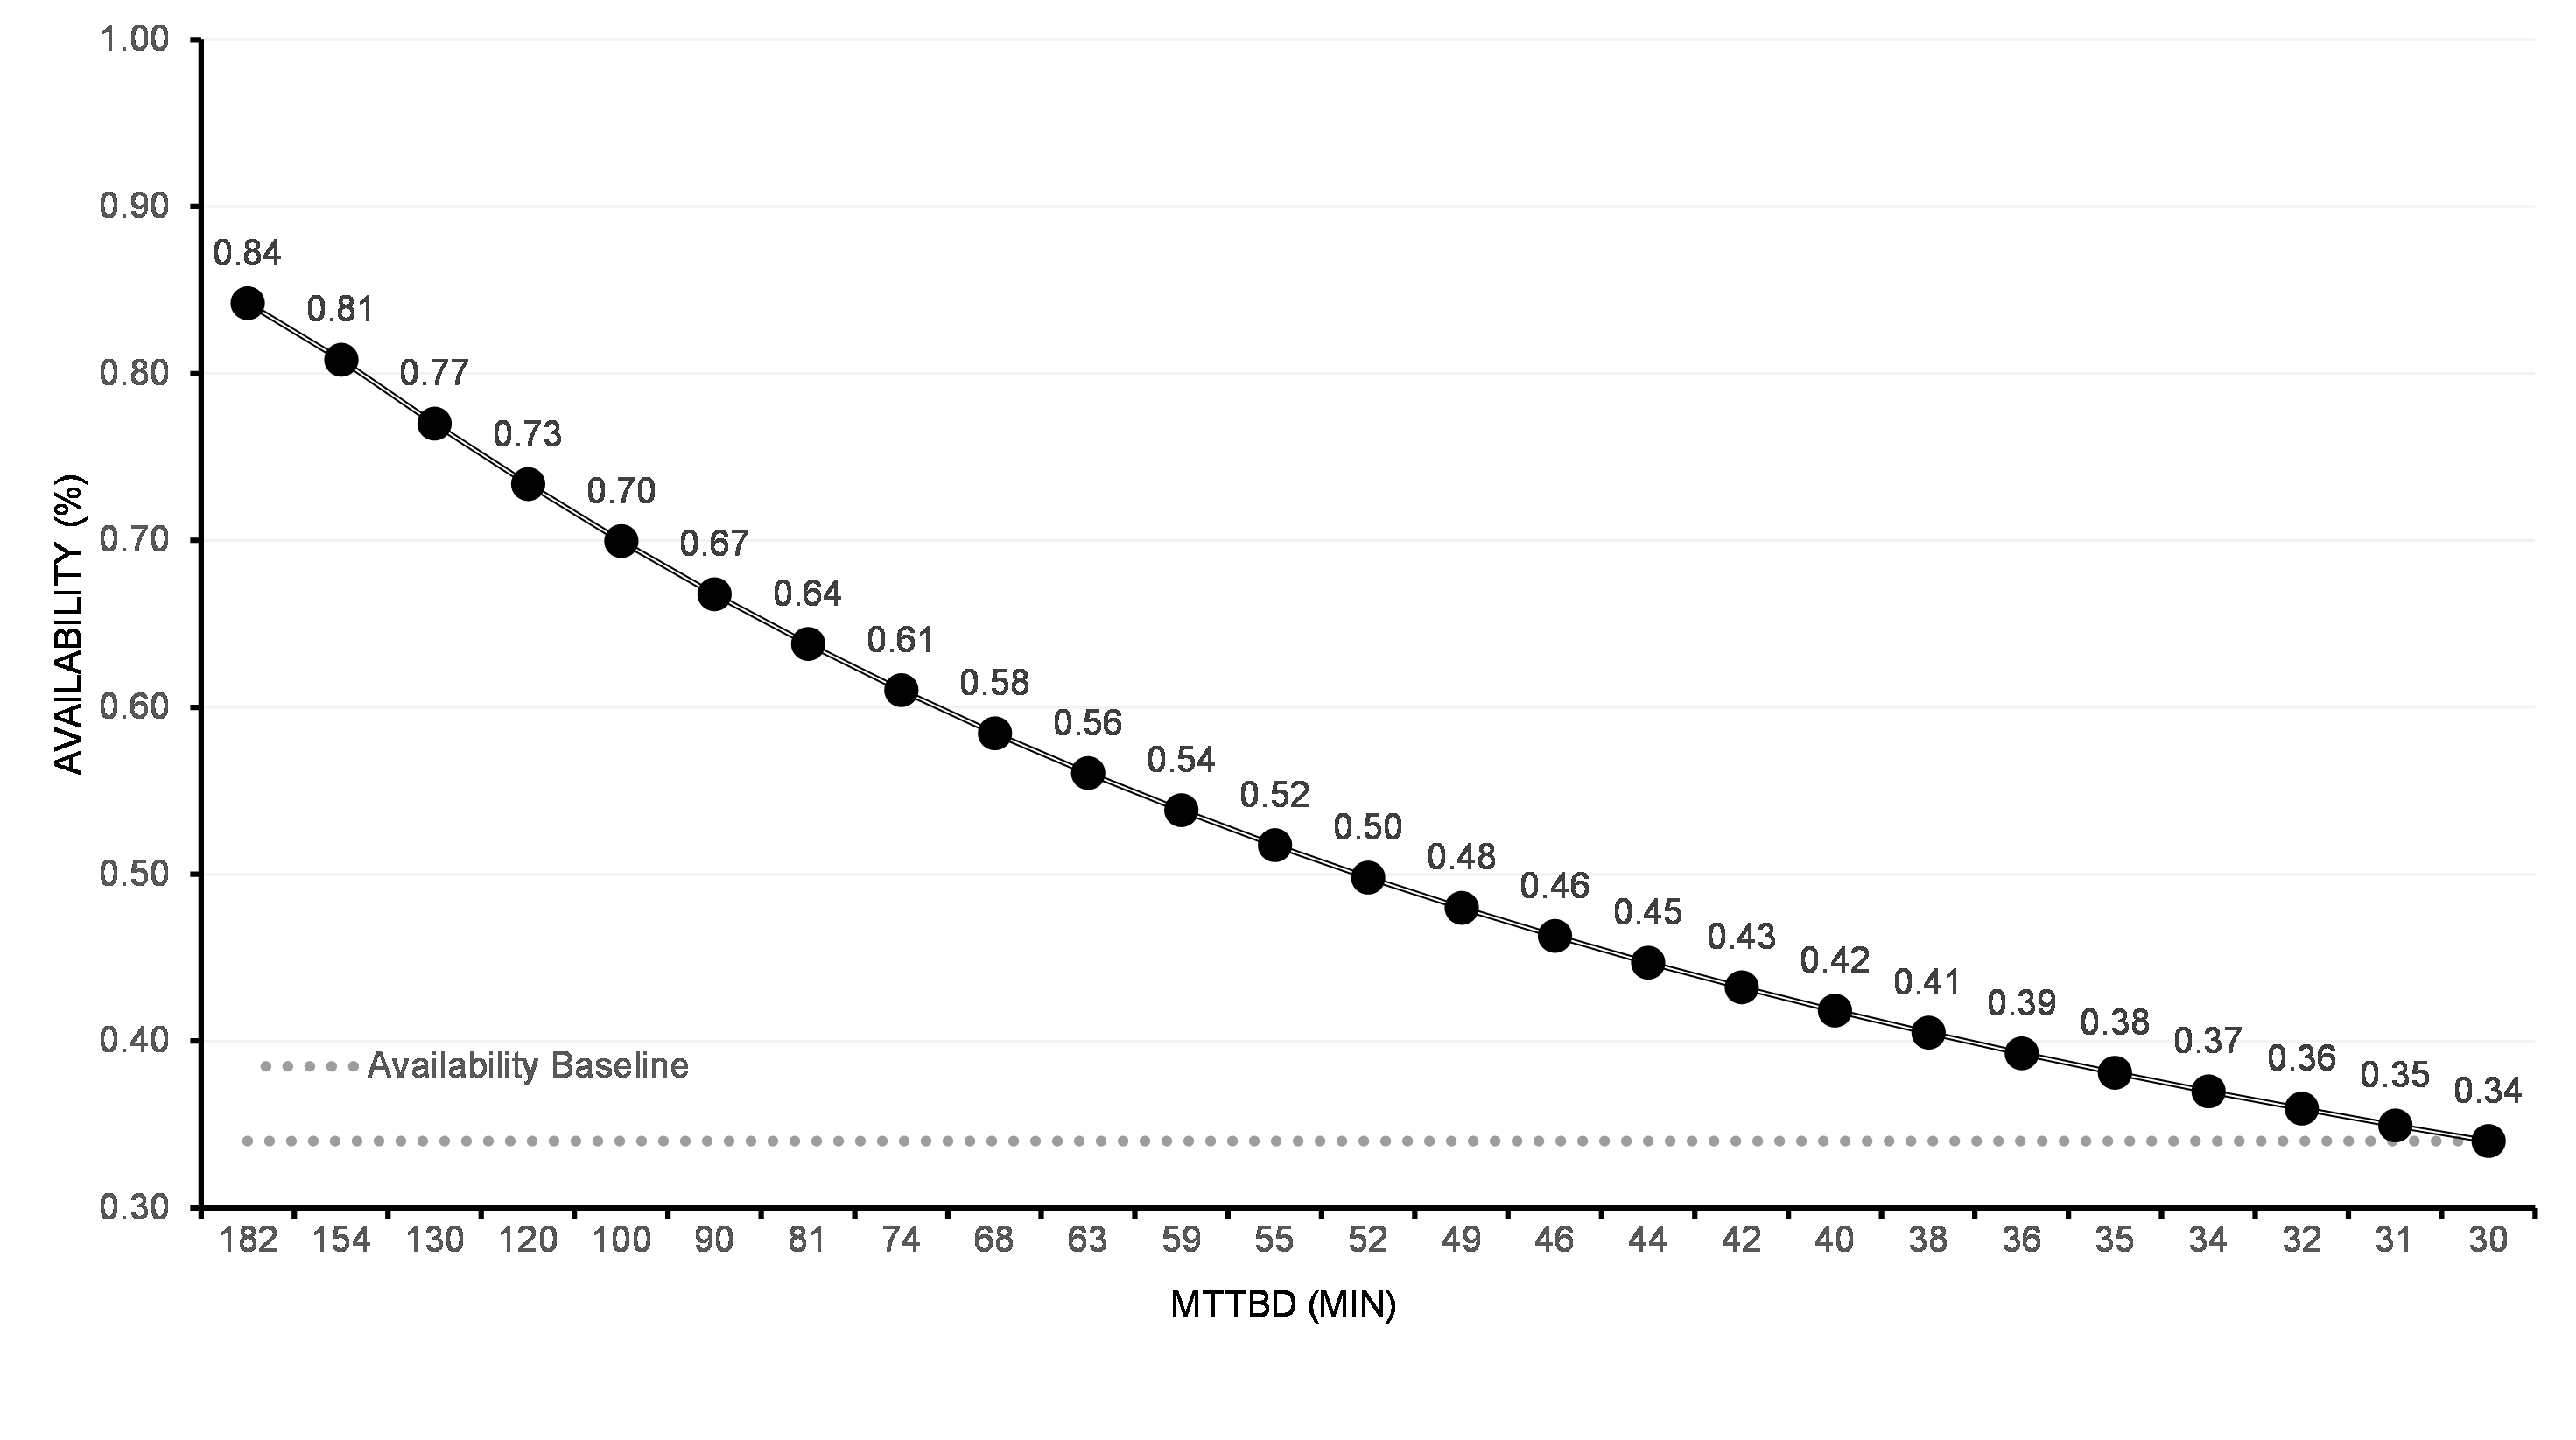
\includegraphics[width=\linewidth]{img/exps/SA_007.png}
         \caption{}
         \label{fig:ctmc_sa_bd}
     \end{subfigure}
     \hfill
     \begin{subfigure}[b]{0.45\textwidth}
         \centering
         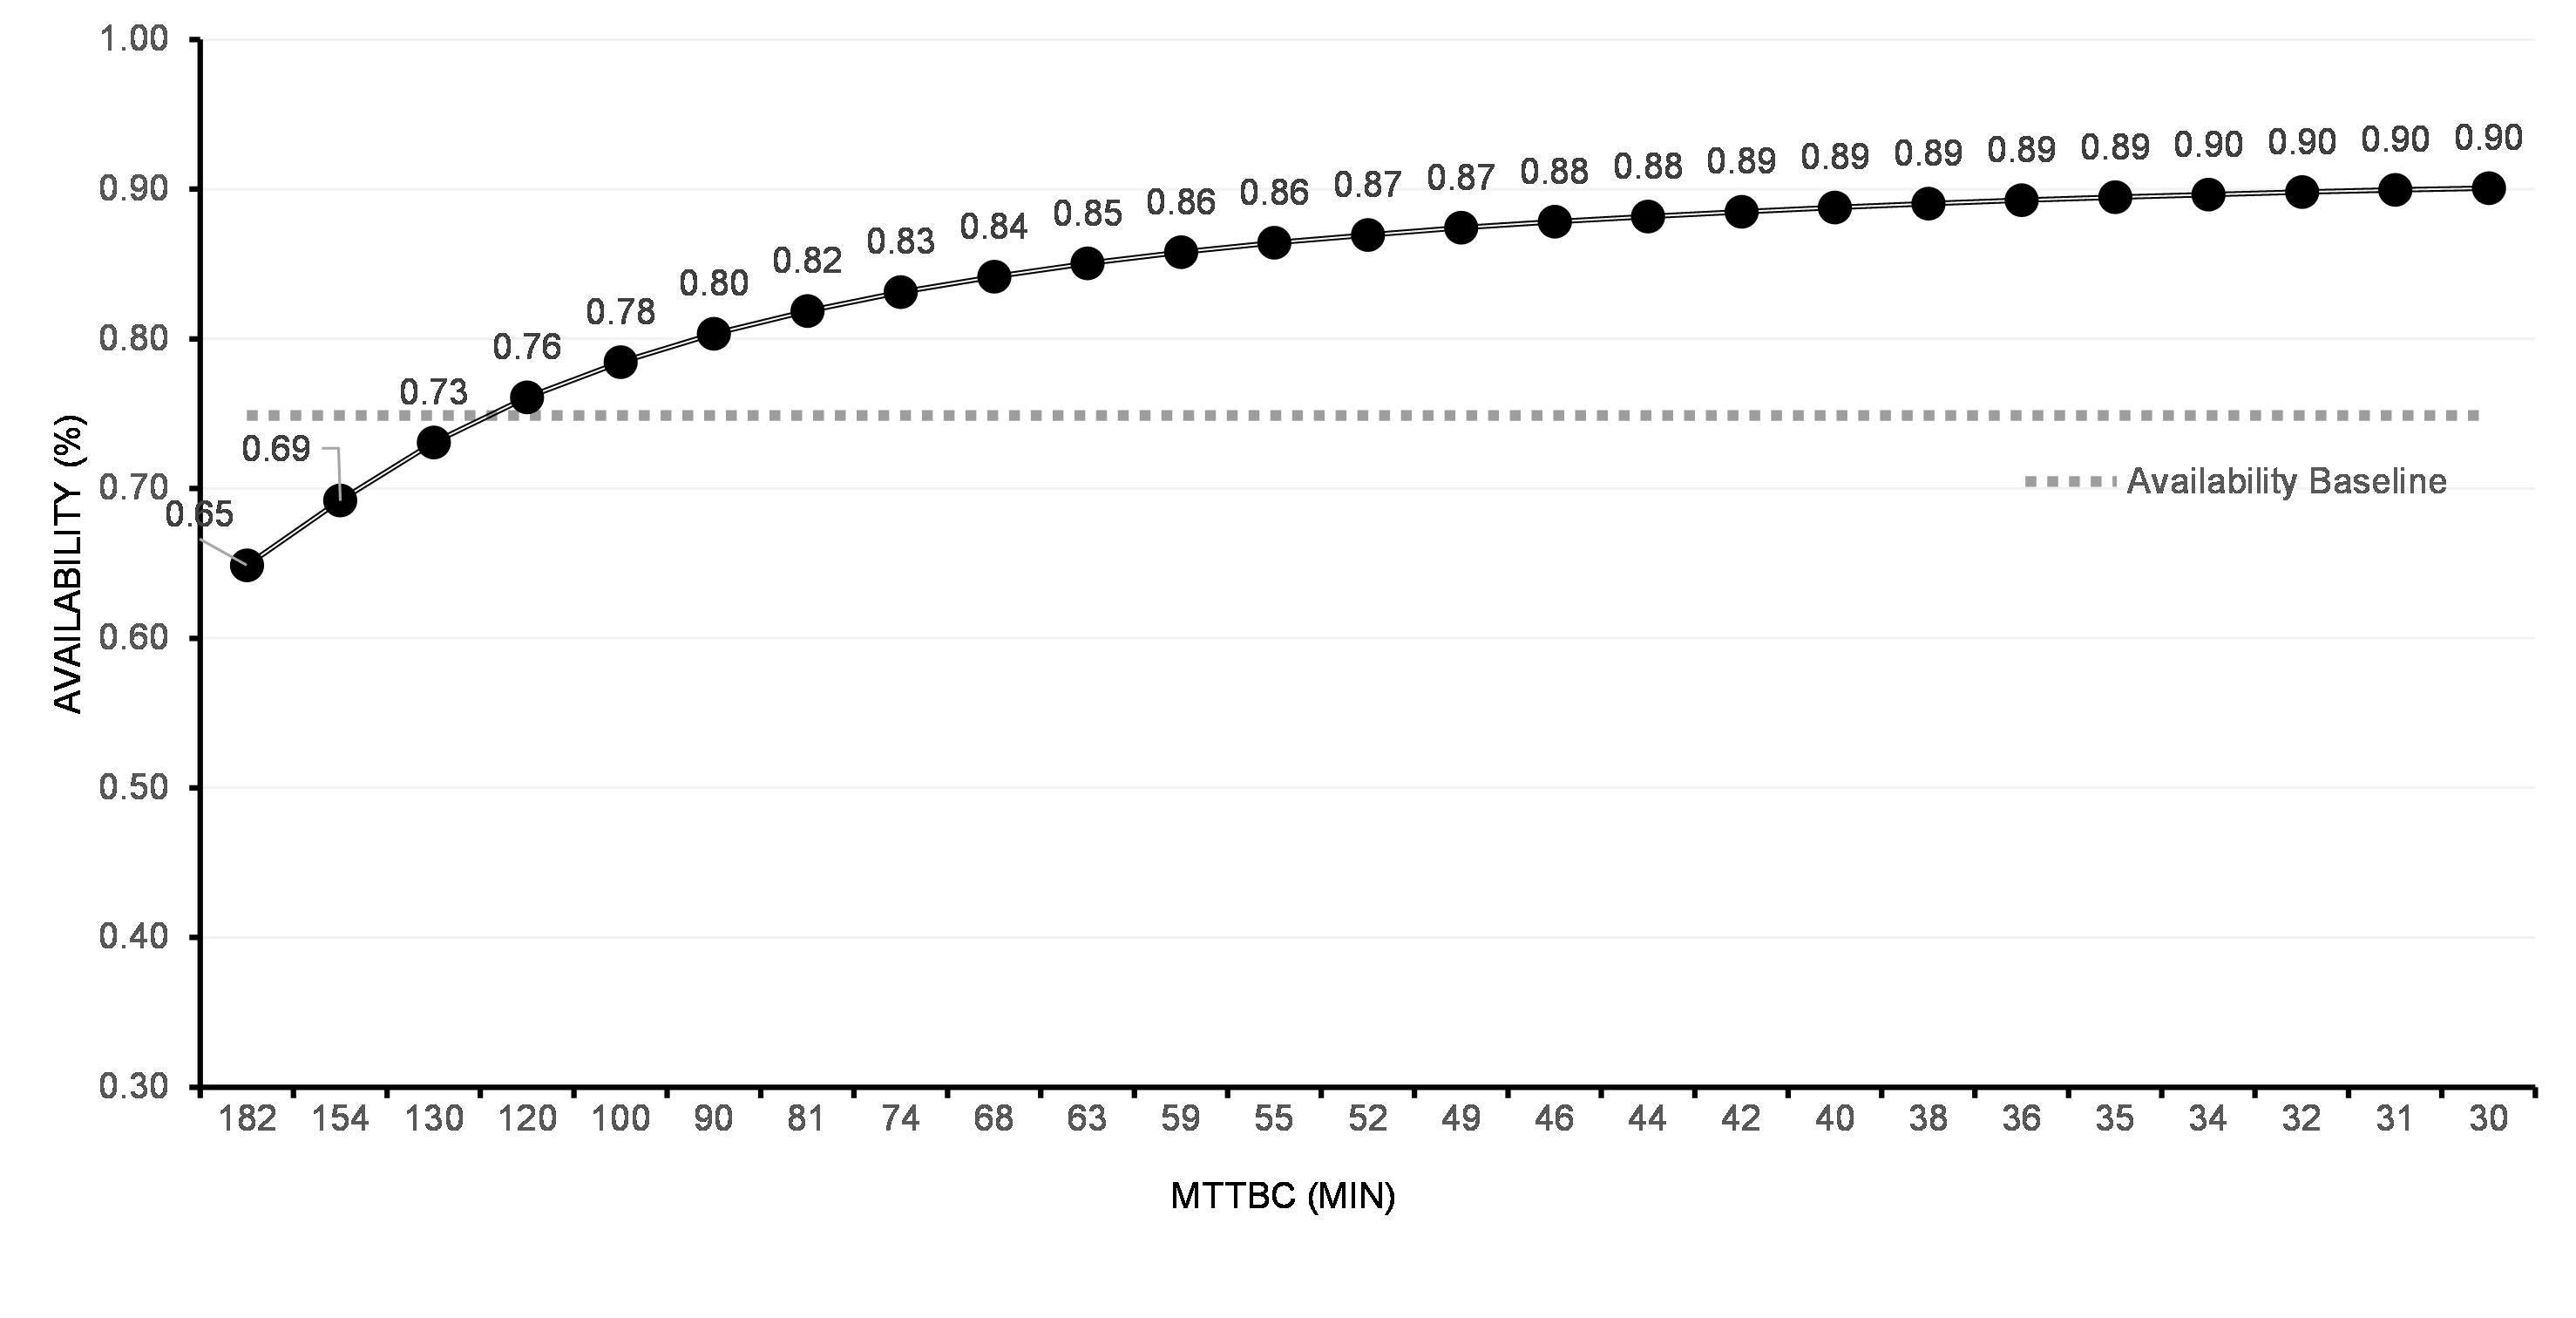
\includegraphics[width=\linewidth]{img/exps/SA_001.png}
         \caption{}
         \label{fig:ctmc_sa_bc}
     \end{subfigure}
     \hfill
     \begin{subfigure}[b]{0.45\textwidth}
         \centering
         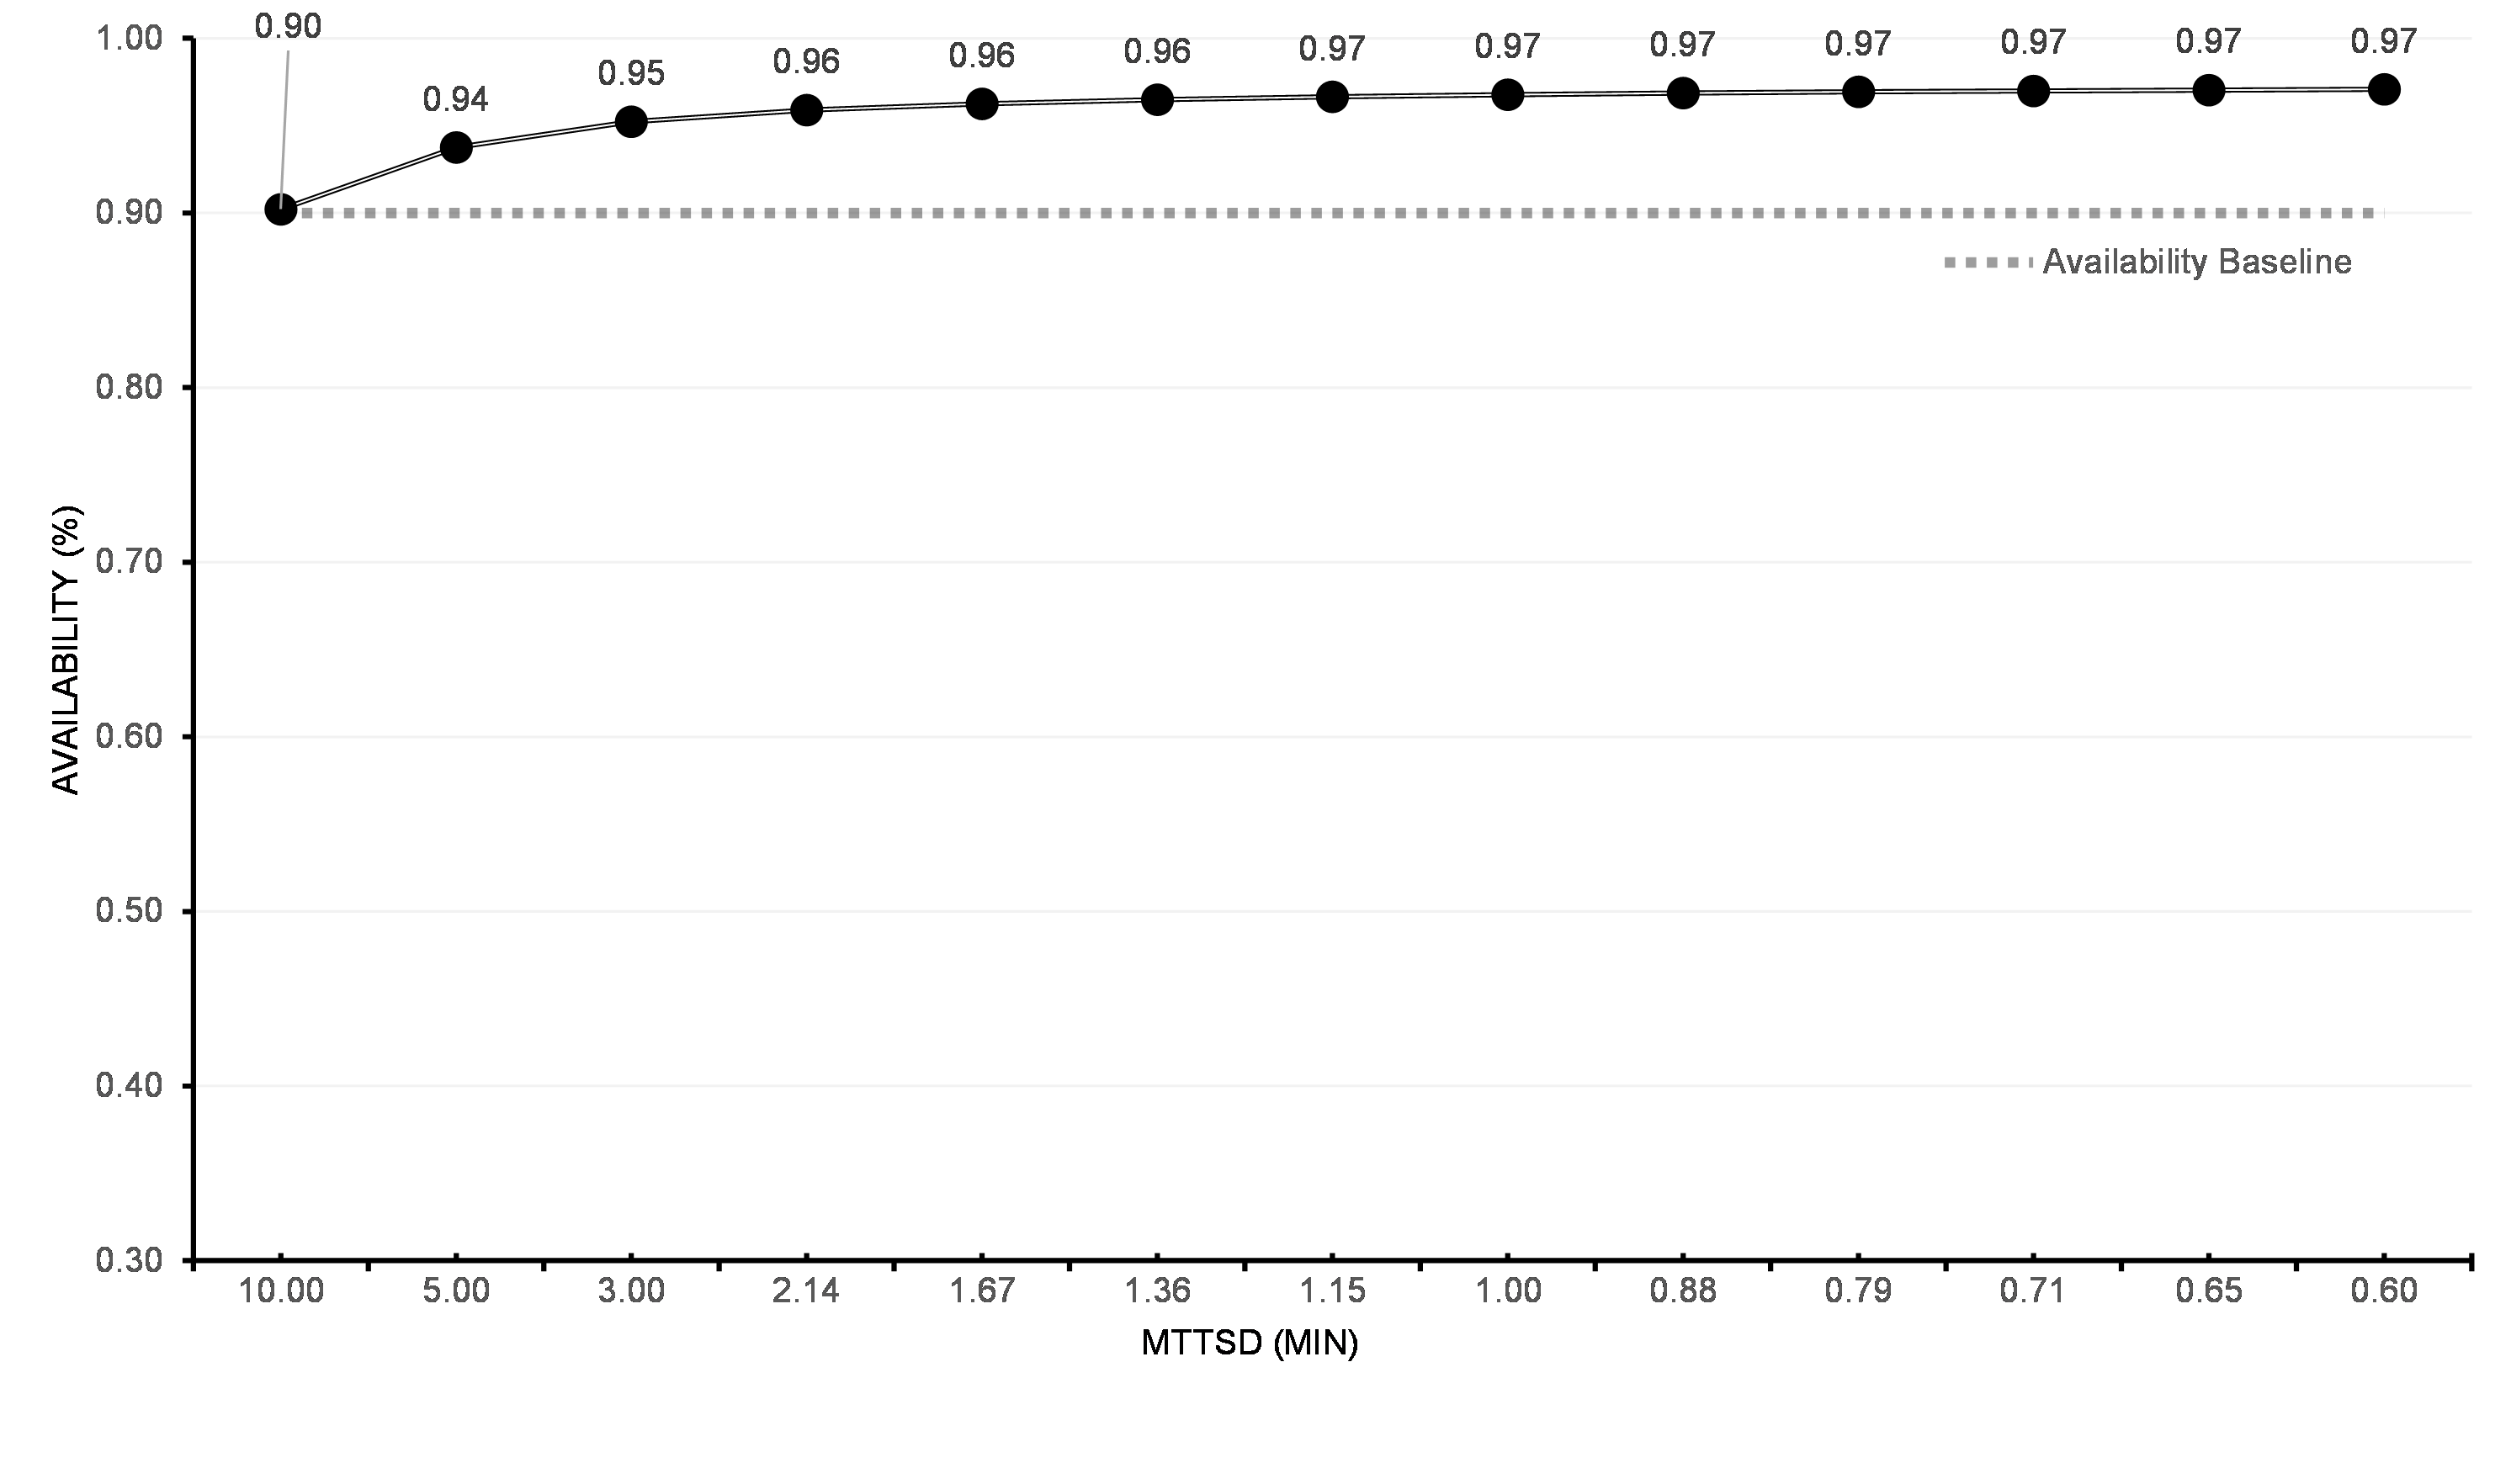
\includegraphics[width=\linewidth]{img/exps/SA_002.png}
         \caption{}
         \label{fig:ctmc_sa_suav}
     \end{subfigure}
        \caption{Variation one by one}
        \label{fig:ctmc_sa}
\end{figure}


Figure \ref{fig:ctmc_sa_bd} shows the graph of variation of $\lambda_{bd}$. The baseline system's availability is represented by $\lambda_{bd}$ equal to 2 discharges per hour or 30 minutes of flight as on the chart (in minutes). By improving the flight time of the UAV device, we can go from the availability of 0.34\% of the time to 0.84\% with 180 minutes of flight (3 hours). 

The variation graph (Fig. \ref{fig:ctmc_sa_bc}) (charging time) shows an availability improvement of about nine (0.90\%) with 30 minutes of charging and a flight time fixed at 90 minutes. Finally, we achieved an availability of 0.97\% in a UAV exchange of fewer than 1.30 minutes (Fig. \ref{fig:ctmc_sa_suav}).



\subsection{Case Study 2}\label{sec:case_studies_sub02}

\begin{figure}[htbp]
\centerline{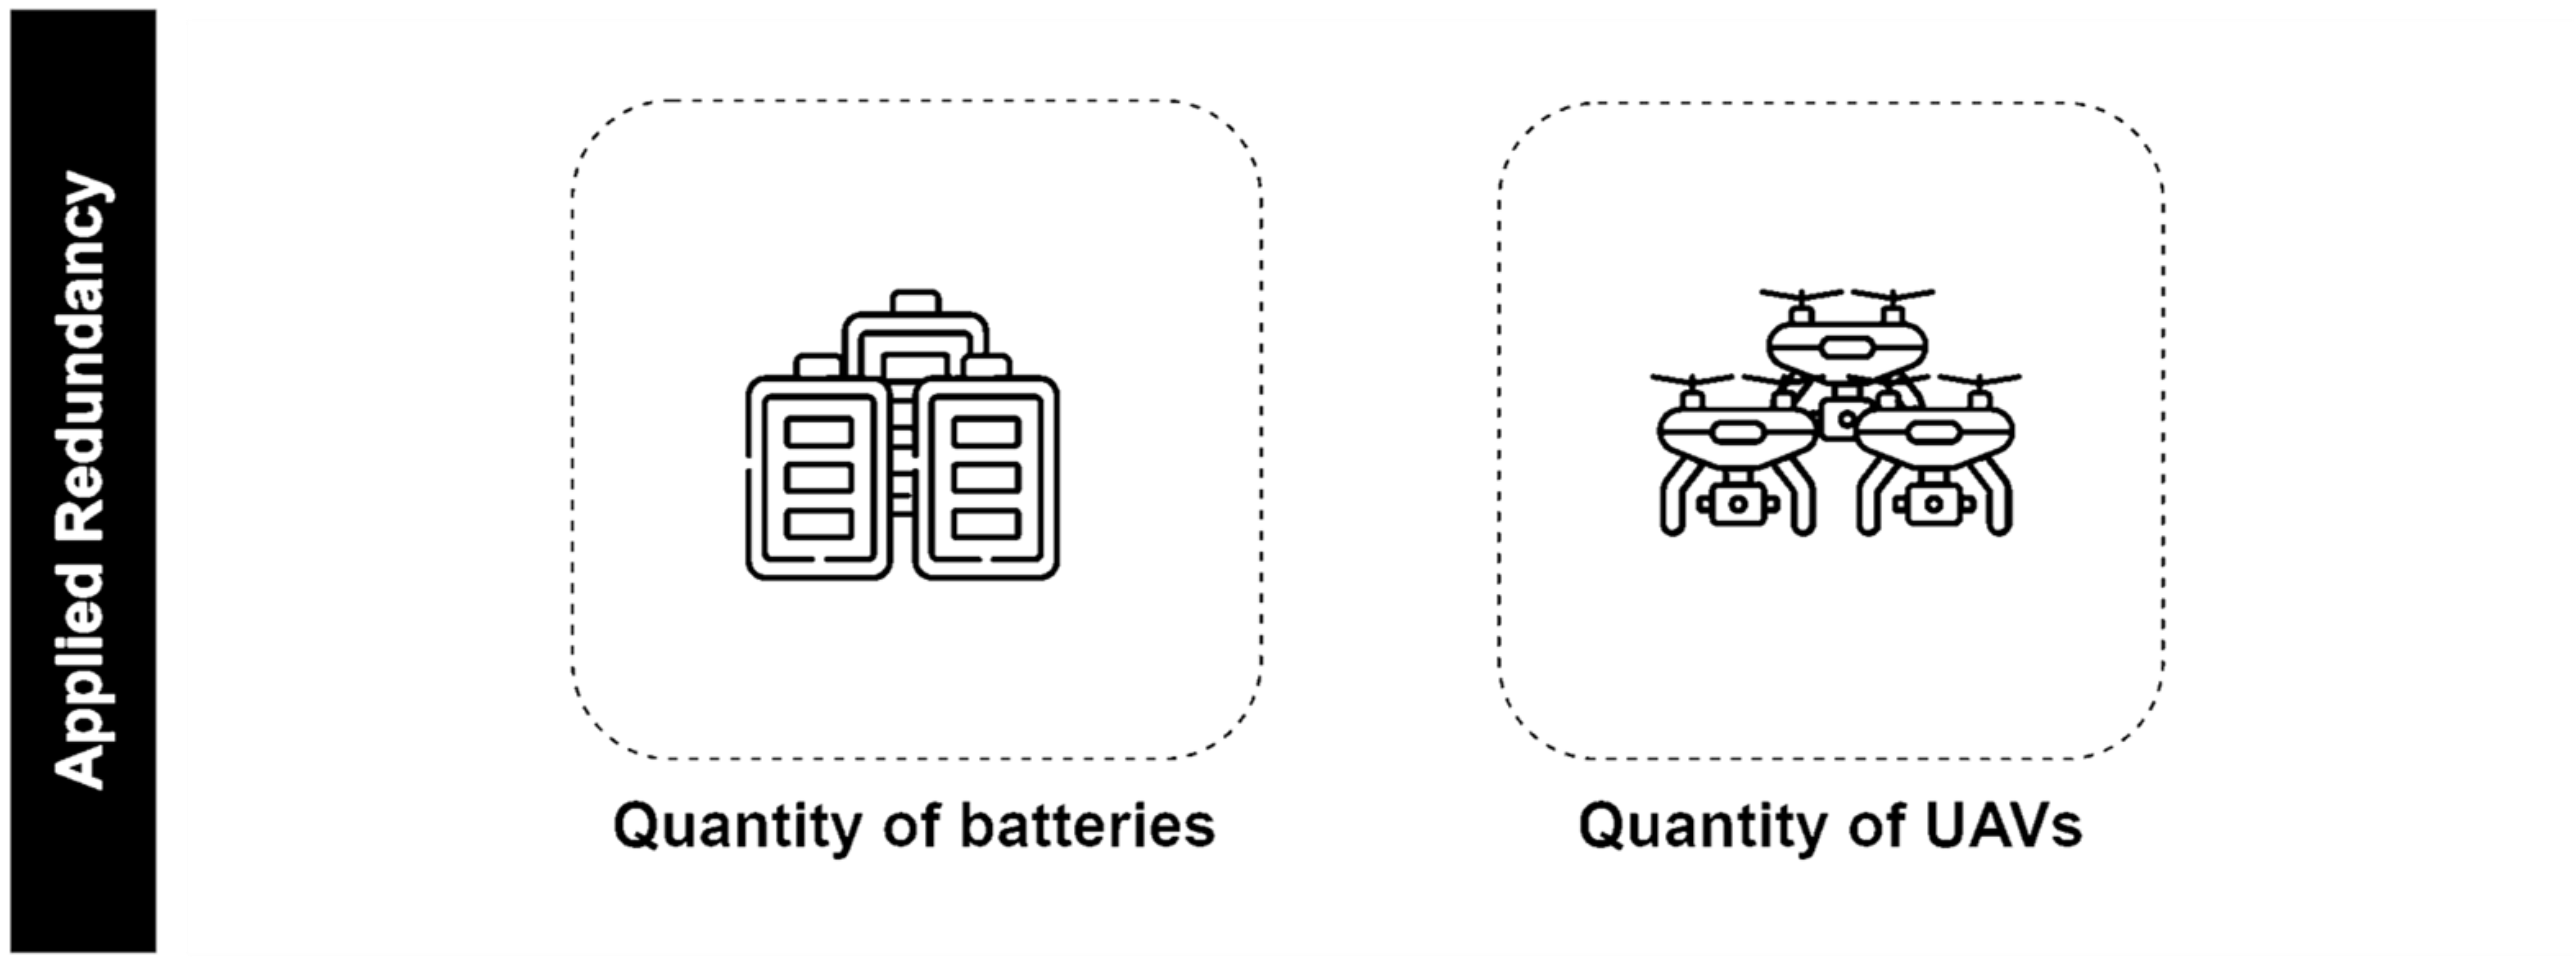
\includegraphics[scale=0.22]{img/operating_model_study_02.png}}
\caption{Applied Redundancy.}
\label{fig:case_study_02}
\end{figure}

To generate models with redundancy techniques using continuous-time Markov chains (CTMC) or even analytical models with equations, we would have to face the explosion of states, which makes it challenging to understand the CTMC and manually calculate the generated analytical equations.

In the system's general availability model for the UAV flight system, a stochastic Petri nets (SPN) model facilitates the modeling of systems with redundancy mechanisms. SPNs are numerical models evaluated by simulation via software. We will use the Mercury tool to evaluate the \citep{maciel2017mercury} model for this study.

The values of input parameters of the SPNs are given by times (MTTs). Table \ref{tab:basic_spn_parameter_values} shows the MTTs of the baseline system composed of the same values of Case Study 1 in time format.


\begin{table}[htbp]
\caption{Parameter values for the SPN model}
\begin{center}
\begin{tabular}{|c|c|}
\hline
\textbf{\textit{Parameter}} & \textbf{\textit{Value (hours)}} \\
\hline
  MTTFD & 5000\\
 MTTRD & 2\\
 MTTBD & 0.5 \\ 
 MTTBC & 2 \\
 MTTSD & 0.166666667 \\
 NB & 1 \\
 ND & 1 \\
\hline
\end{tabular}
\label{tab:basic_spn_parameter_values}
\end{center}
\end{table}

\begin{figure}[htbp]
\centerline{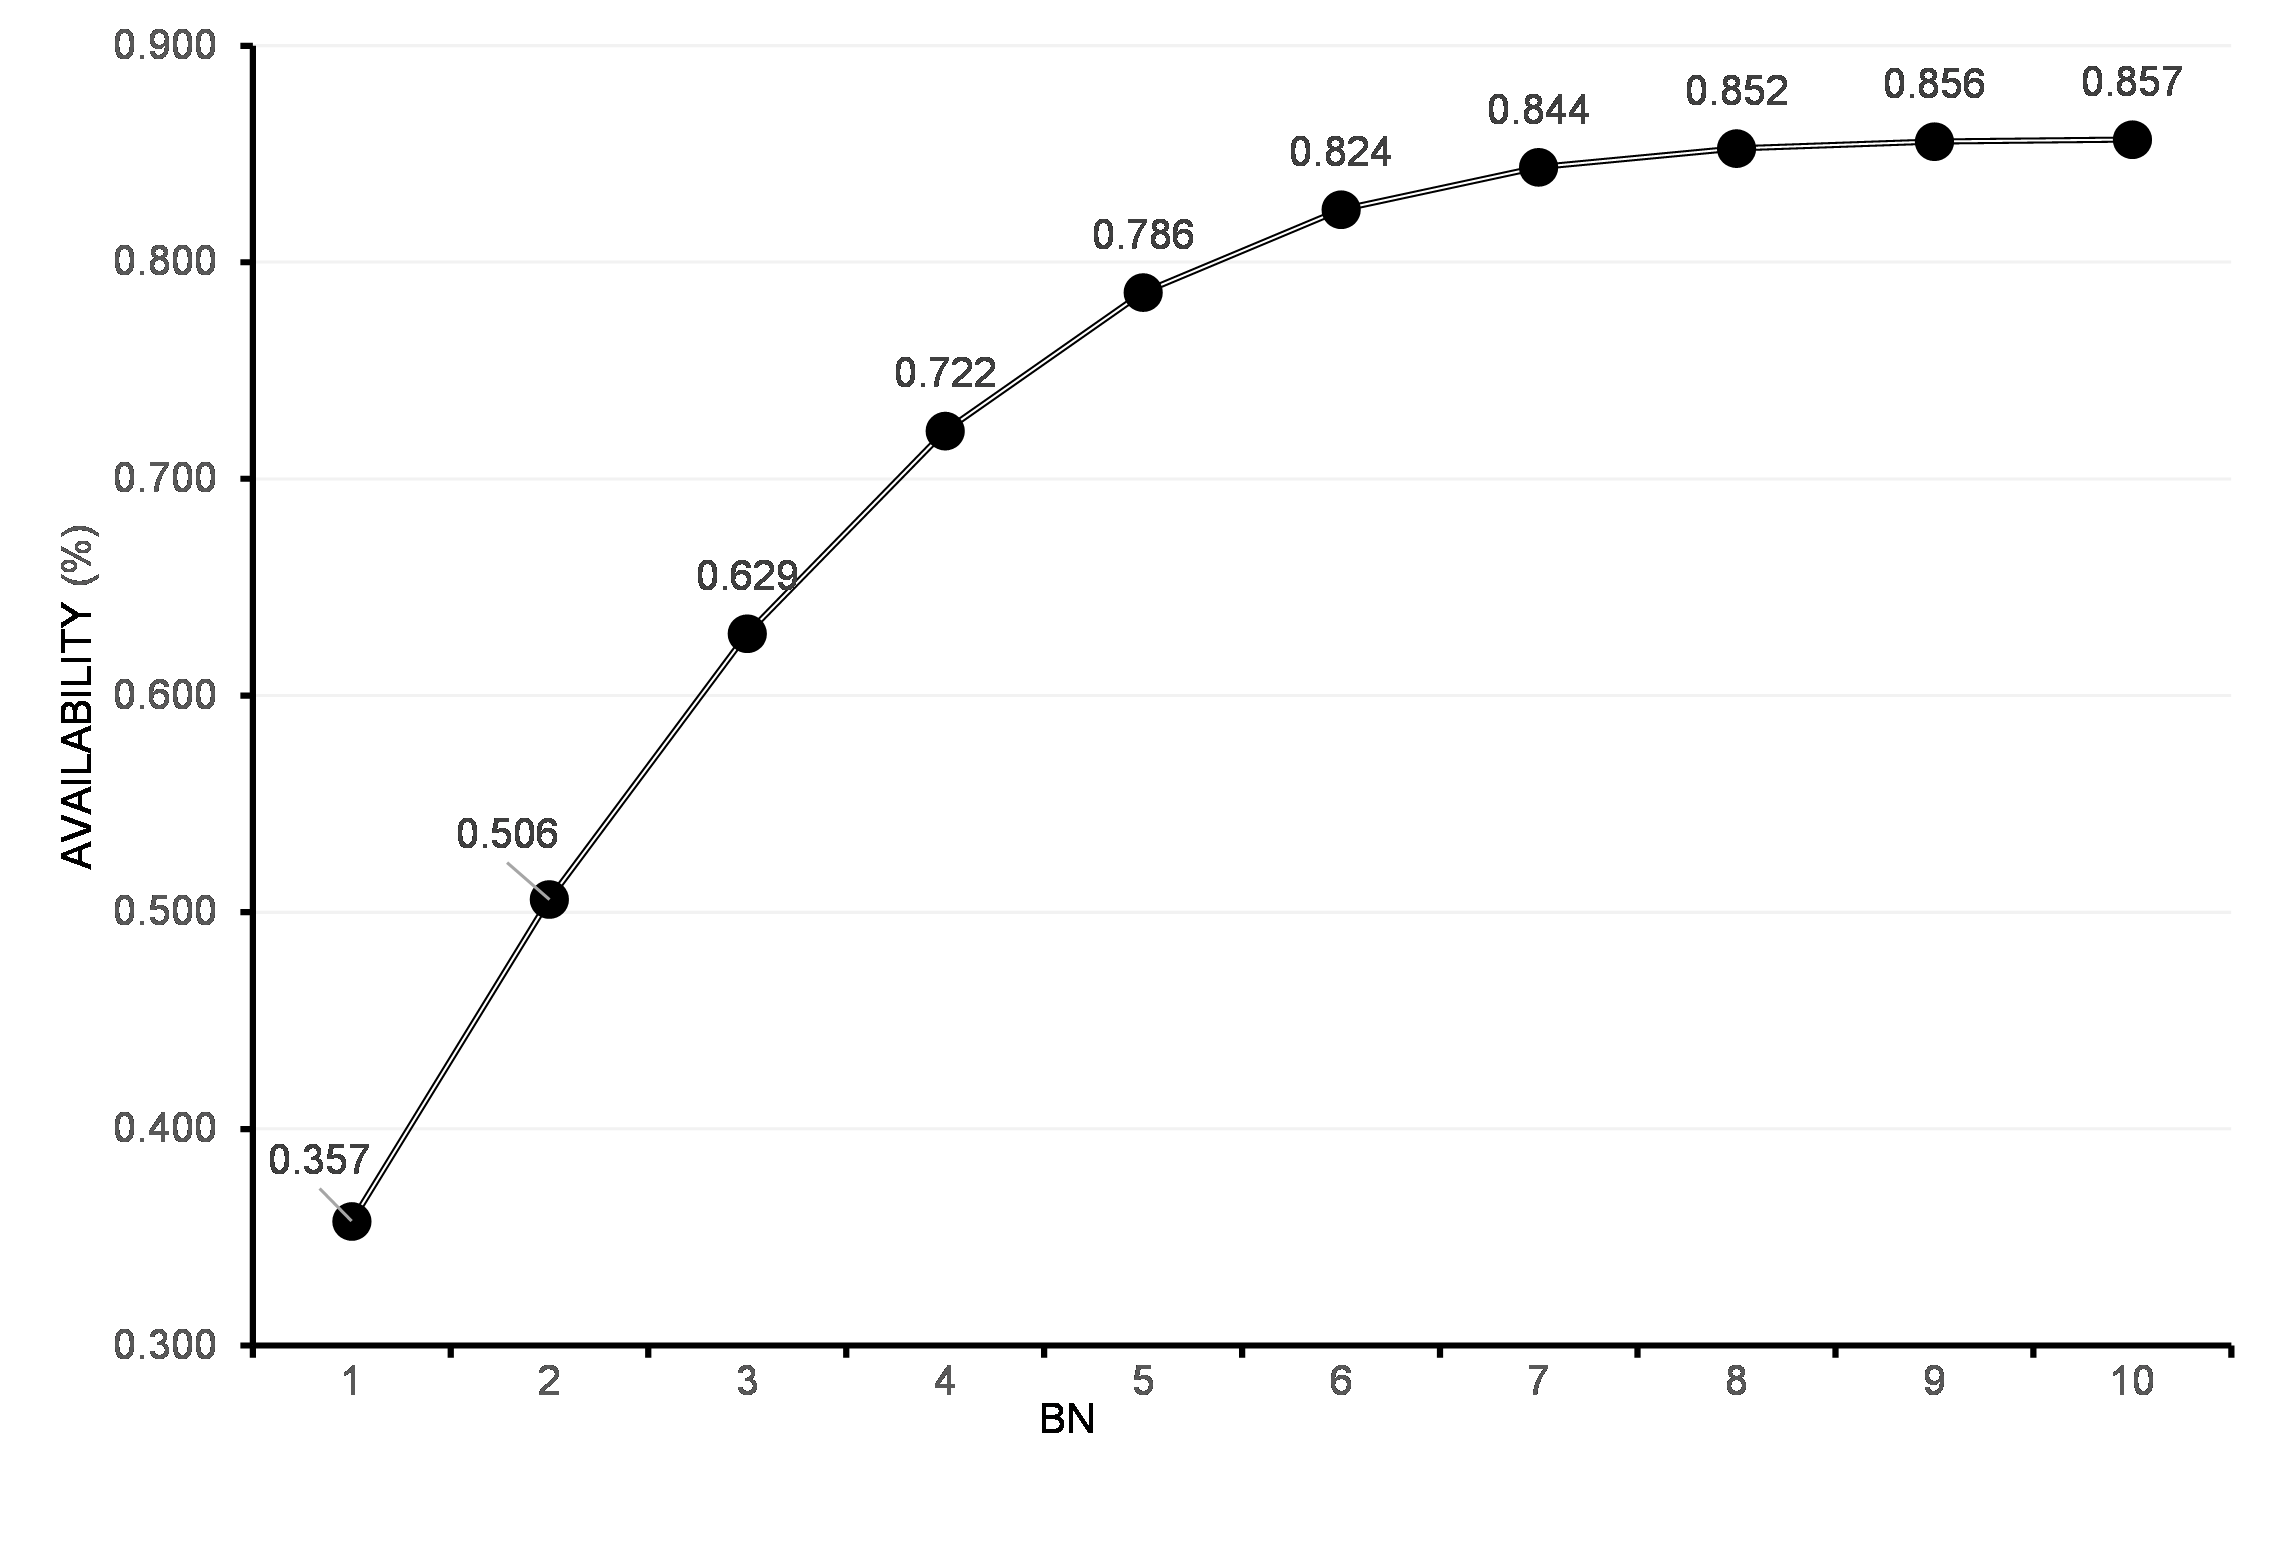
\includegraphics[scale=0.45]{img/exps/SA_006.png}}
\caption{Availability by the number of batteries with basic operating mode MTT parameters}
\label{fig:basic_spn_sa_battery}
\end{figure}

\begin{figure}[htbp]
\centerline{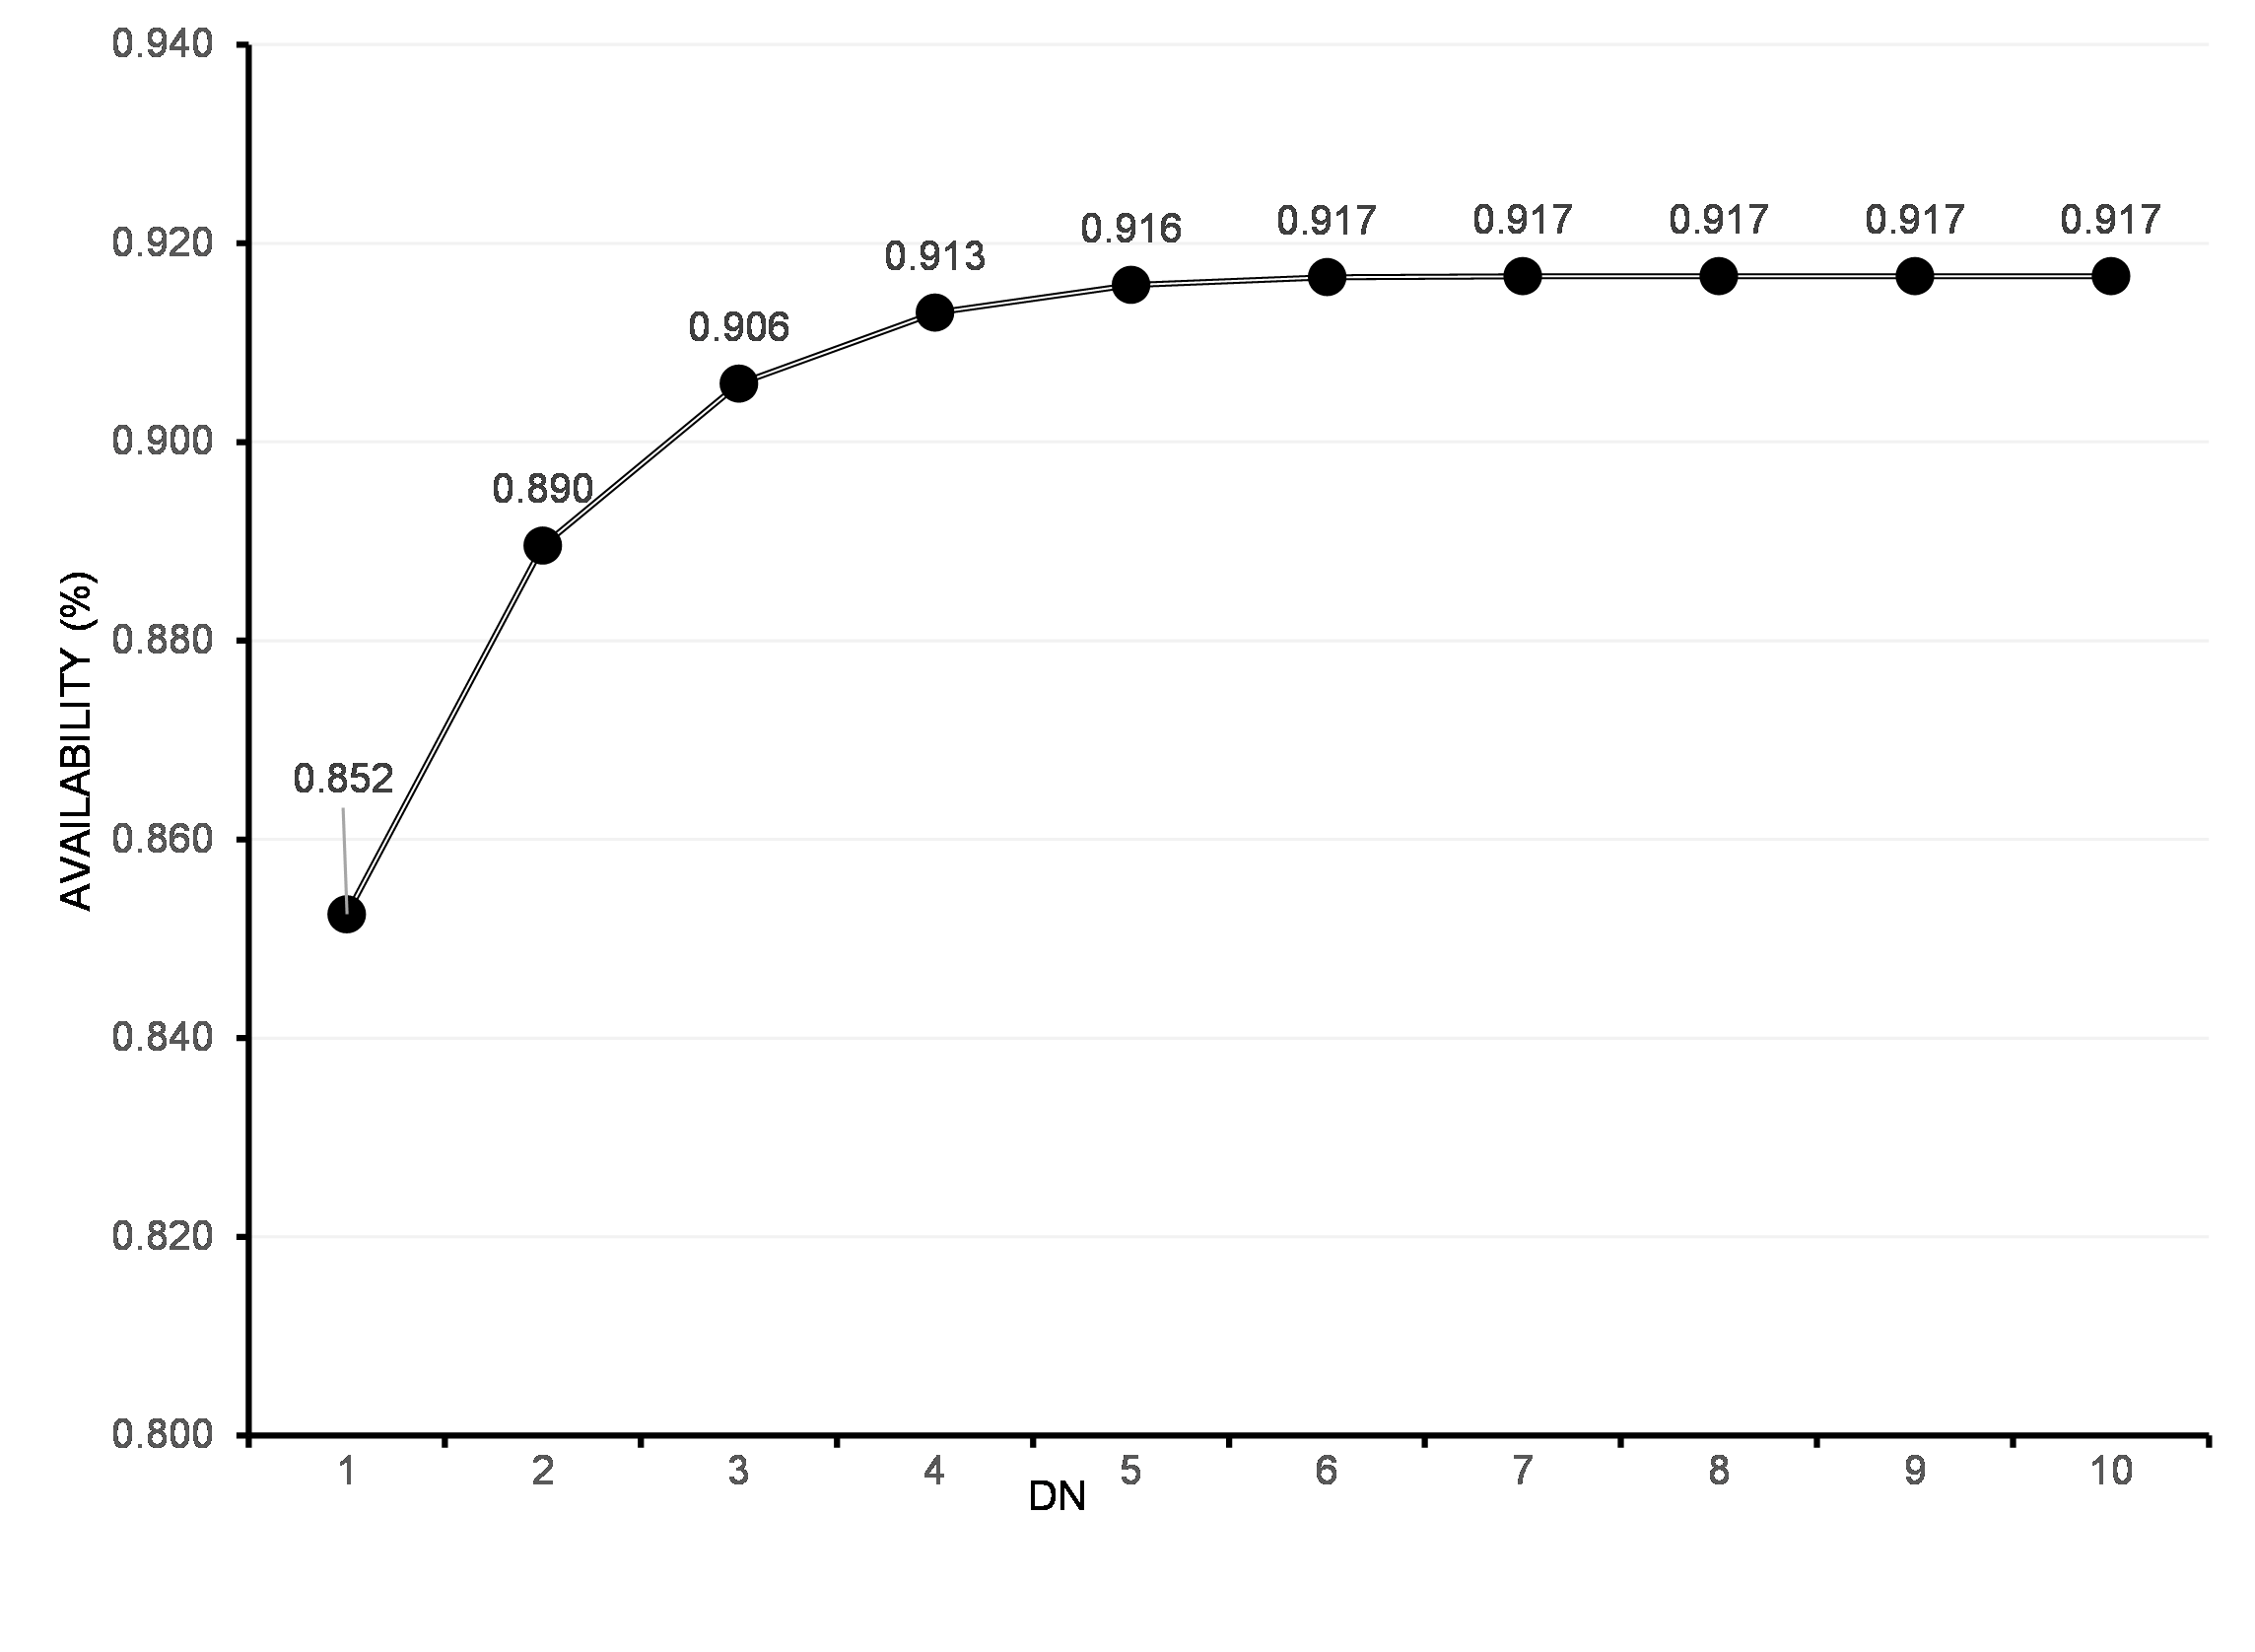
\includegraphics[scale=0.45]{img/exps/SA_003.png}}
\caption{Availability by number of UAVs with basic operating mode MTT parameters}
\label{fig:basic_spn_sa_uav}
\end{figure}


Figure \ref{fig:basic_spn_sa_battery} shows the evolution of the system's general availability only with the application of redundancy in the battery component. We have availability of 0.85\% using 8 spare batteries ready for use.

With the value of spare batteries (NB) set at 8, we vary the value of spare drones (ND) and obtain availability of nine (0.90\%) with 4 spare drones (Fig. \ref{fig:basic_spn_sa_uav}). However, we could not get availability with numbers of nines greater than 0.9\% just by adding redundancy mechanisms or isolated improvements to the baseline system.



\subsection{Case Study 3}\label{sec:case_studies_sub03}

This third case study combines the previous two. The redundancy variations in the battery and UAV components operating mode MTT parameters will be evaluated using improved parameters from Case Study 1 to achieve availability greater than nine. The enhanced parameter values used as input are defined in Table \ref{tab:spn_parameter_values}.

\begin{table}[htbp]
\caption{Improved parameter values for the SPN model}
\begin{center}
\begin{tabular}{|c|c|}
\hline
\textbf{\textit{Parameter}} & \textbf{\textit{Value (hours)}} \\
\hline
  MTTFD & 5000\\
 MTTRD & 2\\
 MTTBD & 2 \\ 
 MTTBC & 0.5 \\
 MTTSD & 0.016666667 \\
 NB & 1 \\
 ND & 1 \\
\hline
\end{tabular}
\label{tab:spn_parameter_values}
\end{center}
\end{table}

\begin{figure}[htbp]
\centerline{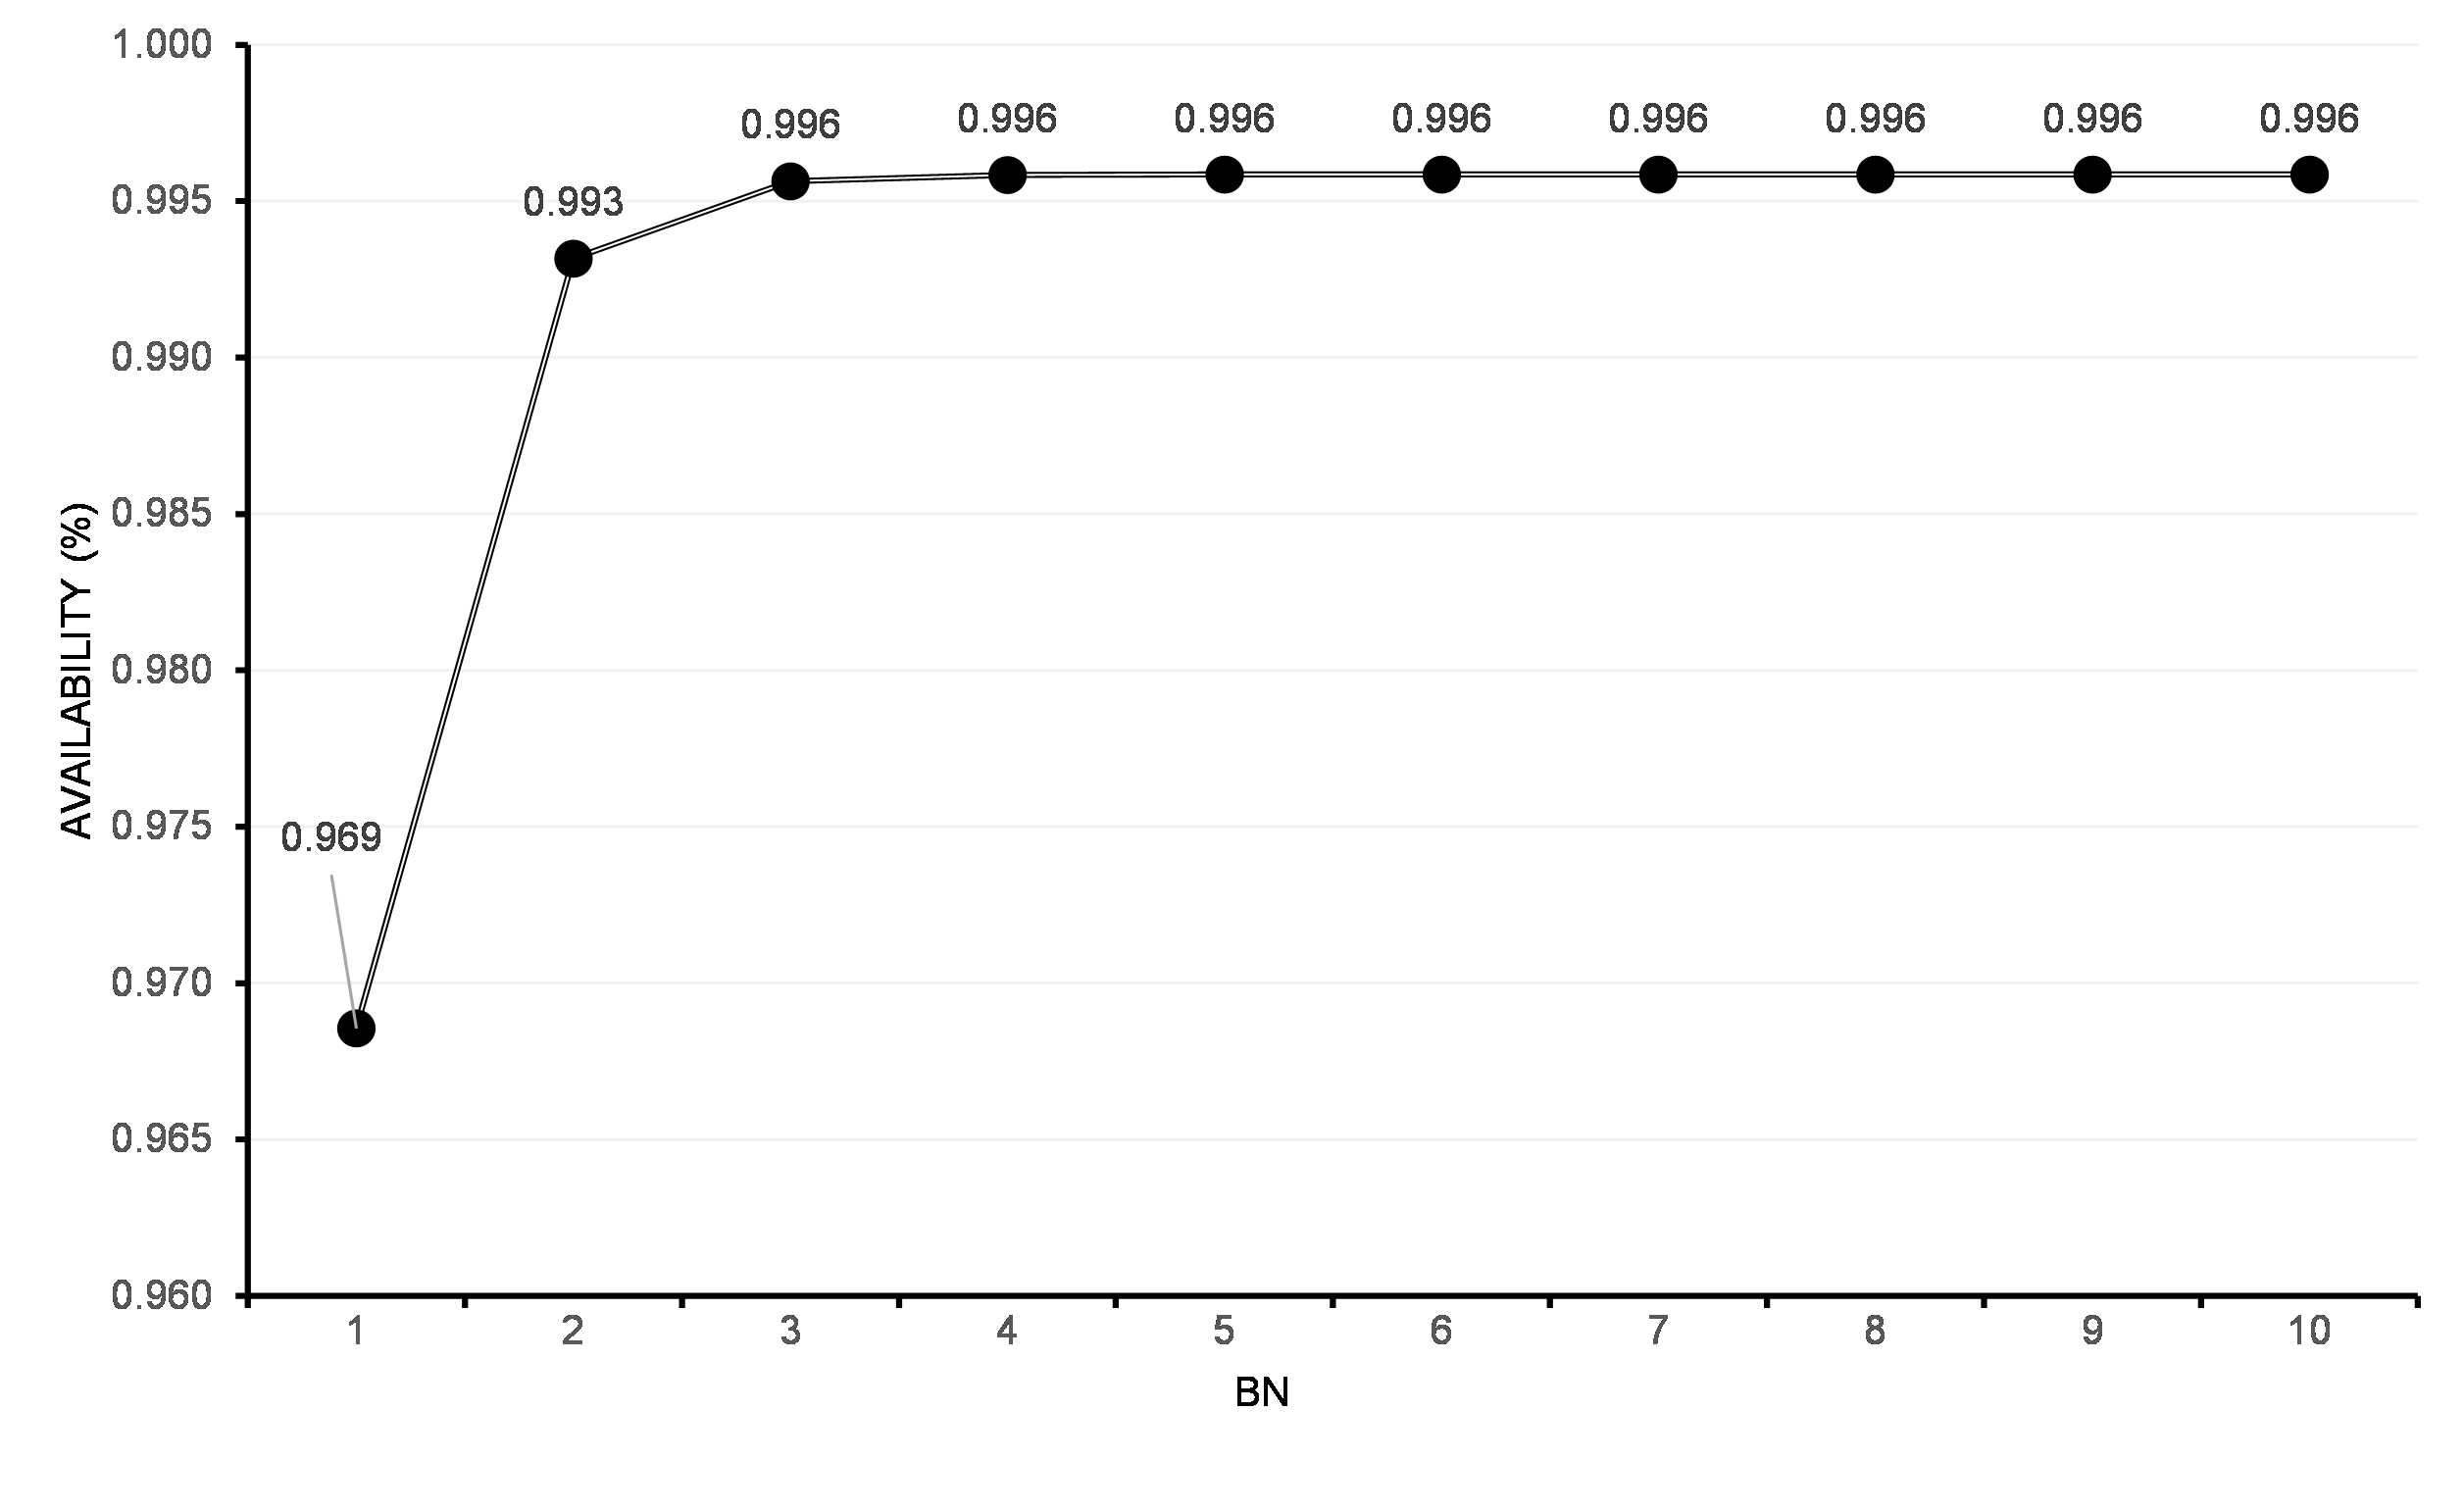
\includegraphics[scale=0.4]{img/exps/SA_005.png}}
\caption{Availability by the number of batteries with improved MTT parameters}
\label{fig:spn_sa_battery}
\end{figure}


\begin{figure}[htbp]
\centerline{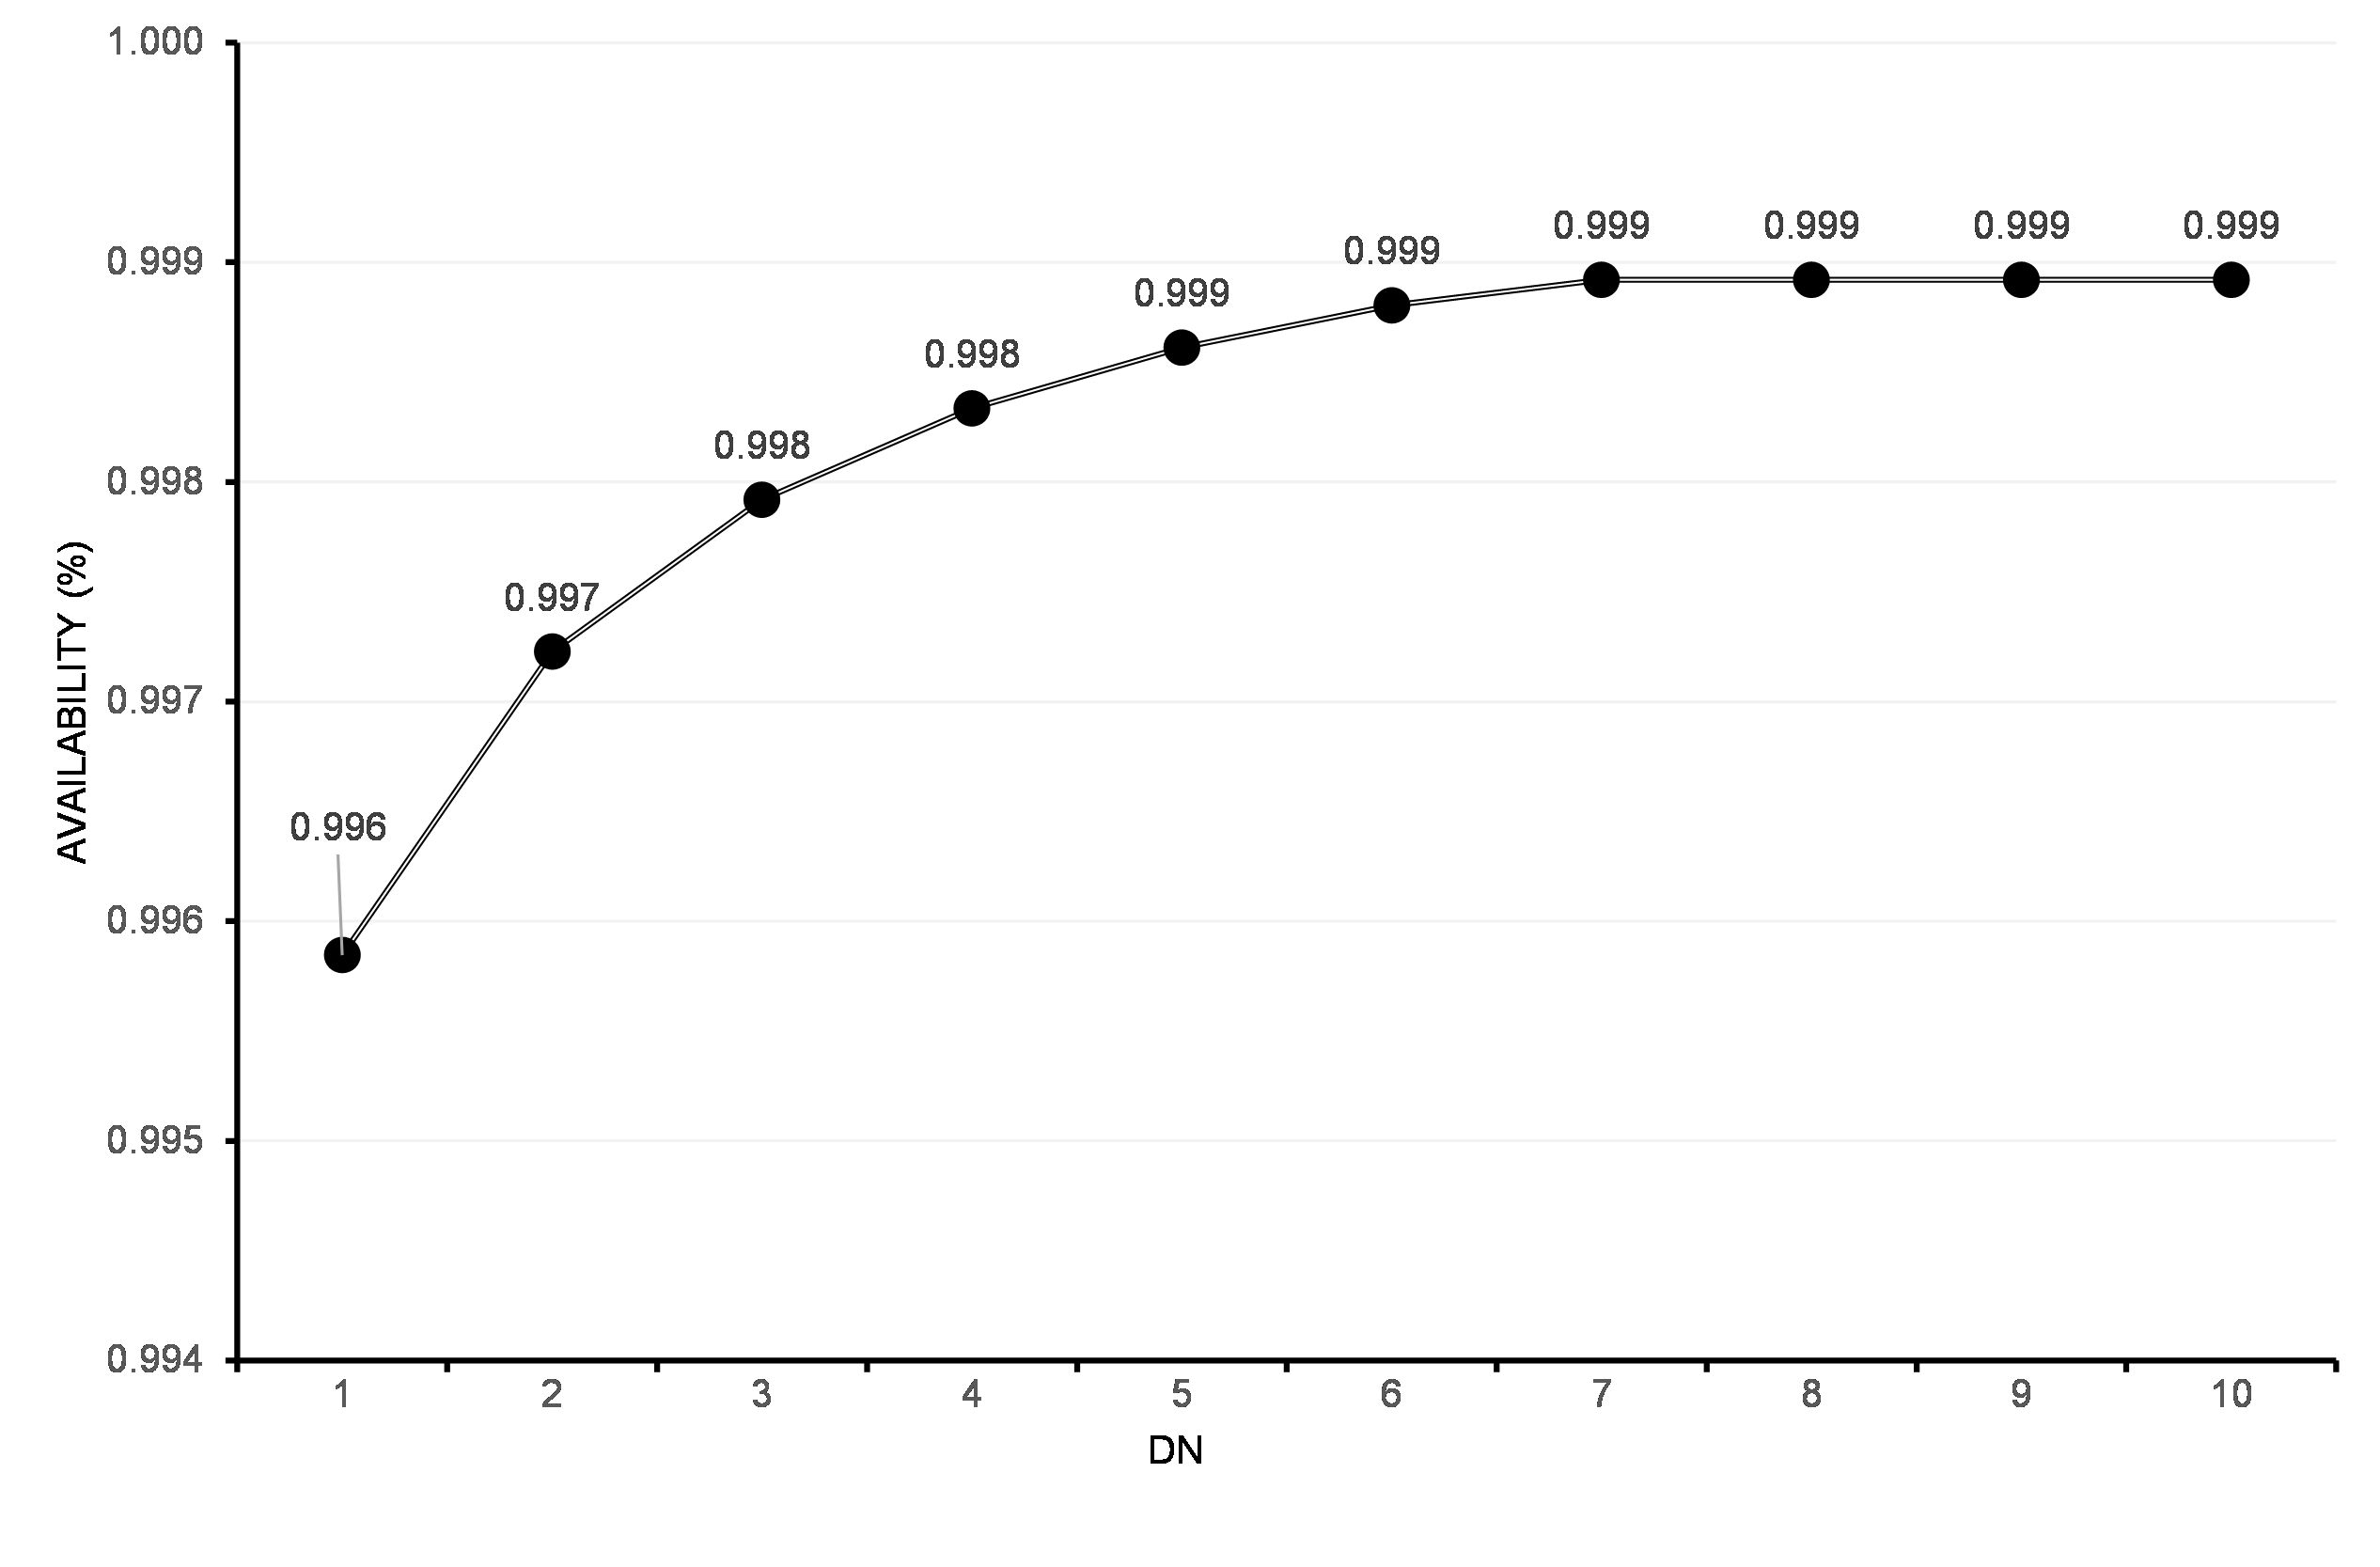
\includegraphics[scale=0.4]{img/exps/SA_004.png}}
\caption{Availability by number of UAVs with improved MTT parameters}
\label{fig:spn_sa_uav}
\end{figure}

At first, it is clear that it was possible to obtain availability with a number of nines equal to 2 only with the addition of an extra battery (Fig.\ref{fig:spn_sa_battery}), with initial availability of improved parameters from the study of case 1 of 0.97\%.

Finally, Figure \ref{fig:spn_sa_uav} shows the graph of the variation in the use of extra UAV devices for redundancy, reaching an availability of 3 nines (0.999\%) with 4 extra UAVs. 

The use of fewer UAVs and spare batteries compared to the previous study can represent a considerable discount on the final budget of a system with these characteristics.




\section{Conclusions and future work}\label{sec:conclusions}

This work proposes two models for evaluating the availability of critical monitoring systems implemented in UAV devices. In three case studies, an assessment of the system's availability has been carried out, given the improvements made and the models used. 

The first case study varies baseline system time parameters symbolizing component improvements. The improvements had a limited availability of 0.97\%. In the second case study, using redundancy mechanisms and a Petri net model with the same baseline, the availability improvement was limited to 0.91\% with 8 batteries and 6 spare UAVs. In the last case study, there was a significant improvement in availability, benefiting from improvements in the components with the joint use of redundancy mechanisms, which allowed an overall availability of the system of the order of 3 nines, 0.999\%.

In future work, we intend to evaluate the cost vs availability metrics of the case studies performed and perform an availability comparison of this type of system implemented in the cloud, fog, and edge computing paradigms.


\section*{Acknowledgment}\label{sec:acknowledgment}
The authors would like to thank the Brazilian government for financial support through the Fundação de Amparo a Ciência e Tecnologia de Pernambuco (FACEPE), Modeling Distributed and Concurrent Systems (MoDCS) group for helping to improve this research.


\bibliographystyle{plainnat}
\bibliography{references}


\end{document}